\documentclass[acmsmall, natbib=false, nonacm]{acmart}
\usepackage{natbib}
\usepackage[T1]{fontenc}
\usepackage[french]{babel}
\usepackage[autolanguage]{numprint}
\bibliographystyle{unsrtnat}
\usepackage{tabularx} % extra features for tabular environment
\usepackage{amsmath}  % improve math presentation
\usepackage{tabto}
\usepackage{amsfonts}
\usepackage{multirow}
\usepackage{caption}
\usepackage{subcaption}
\usepackage{dsfont}
\usepackage{graphicx} % takes care of graphic including machinery
\usepackage[ruled,vlined]{algorithm2e}
\usepackage{float}
%\usepackage[margin=1in,letterpaper]{geometry} % decreases margins
\include{pythonlisting}

%+++++++++++++++++++++++++++++++++++++++
\begin{document}

\title{\textbf{Transport optimal pour la complétion de données manquantes dans des séries temporelles}}
\author{Léo LAFFEACH}
\affiliation{%
  \institution{ENS Rennes}
}
\author{Romain TAVENARD}
\affiliation{%
  \institution{LETG, Université Rennes 2}
}
\date{8 juillet 2022}

\begin{abstract}
Dans ce papier, nous traitons du sujet des données manquantes et abordons des méthodes pour effectuer une complétion.
Nous nous limitons au domaine des séries temporelles et utilisons deux jeux de données provenant de différents domaines et donc qui ont des différences temporelles.
Nous présentons une méthode de complétion de données permettant, en plus d'une association des données, un alignement temporel entre les différents domaines. Cette méthode se nomme \textit{Match-And-Deform} (MAD),
et nous comparons cette méthode à une méthode utilisant la divergence de Sinkhorn.
\end{abstract}
\maketitle

\section{Introduction}
Collecter des données peut facilement s'avérer complexe et il en résulte un grand nombre de données manquantes dans les jeux de données.
C'est un problème qui existe depuis que les scientifiques collectent des données, et c'est un problème de plus en plus récurrent connaissant la large quantité de données collectées.

Il est donc utile d’avoir des méthodes pour compléter ces valeurs manquantes, 
plusieurs approches peuvent être possibles comme compléter avec une valeur constante bien choisie,
ou alors apprendre à imputer.
On va s'inspirer des méthodes présenté dans \textit{Missing Data Imputation using Optimal Transport} [1] qui utilise le transport optimal pour faire des correspondances entre les données d'une même distribution pour les compléter.
Cependant, nous nous intéressons ici à la complétion de jeux de données de séries temporelles et utilisons plusieurs domaines pour effectuer la complétion.
Prenons un exemple:
\begin{figure}[H]
    \centering
    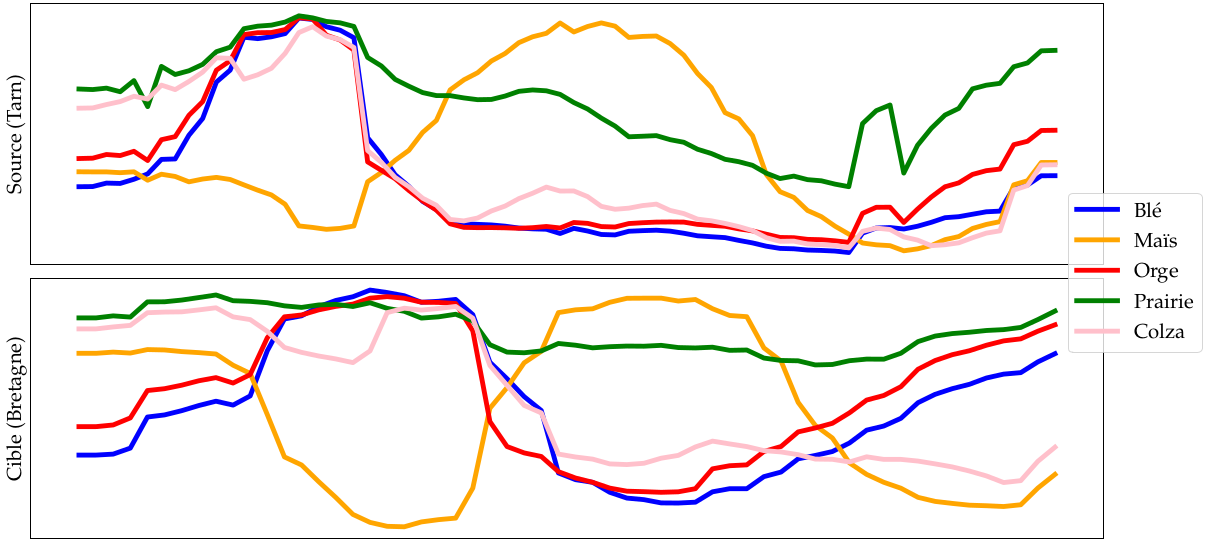
\includegraphics[scale = 0.3]{images/exemple_serie_temps.png}
    \caption{Moyennes par classe d'occupation du sol d'un indicateur de croissance de végétation pour deux zones géographiques différentes.}
    \label{exemple_intro}
\end{figure}
Sur la figure~\ref{exemple_intro}, nous avons l'évolution des moyennes de croissance de végétation dans le Tarn et en Bretagne, 
on remarque que les moyennes semblent avoir une évolution similaire sur les deux domaines, 
mais ces variations apparaissent à des temps différents. 
Par exemple, le maïs semble pousser plus tôt dans le Tarn que en Bretagne alors que le blé et l'orge ont une deuxième croissance plus tôt en Bretagne que dans le Tarn. 
Ainsi, en cas de données manquantes, on pourrait vouloir utiliser ces données similaires pour effectuer une complétion. 
Mais il nous faut alors une méthode pour aligner d'un point de vue temporel les différents \textit{dataset} et ensuite faire correspondre les données pour faire la complétion.
On fait alors face à deux problèmes pour la complétion de données, l'alignement temporel et une assossiation entre les données des différents jeux.
Une des pistes de résolution peut se trouver avec le transport optimal (\textit{Optimal Transport} (OT)), qui permet d'avoir une distance géométriquement sensée pour comparer des distributions discrètes, et donc des données.
L'autre peut voir une solution avec l'alignement temporel dynamique (\textit{Dynamic Time Warping} (DTW)), permettant l'alignement de données temporelles.

Dans la suite du document nous allons d'abord présenter le transport optimal qui sert à la divergence de Sinkhorn,
puis nous allons présenter un algorithme permettant la complétion de données en utilisant cette fonction de coût.
Nous présenterons ensuite notre méthode \textit{Match-And-Deform} (MAD), se basant sur le transport optimal mais aussi sur l'alignement temporel dynamique.
Et enfin nous comparons les différentes méthodes sur quelques couples de domaines.

\section{Transport Optimal et imputation de données manquantes}
Ici nous introduisons le transport optimal. Il définit une distance entre deux distributions.
Pour coller aux conventions habituelles, on suppose que \textbf{X} est de dimension $(n, d)$.
\subsection{Transport Optimal}
Le transport optimal est un problème d’optimisation qui permet de définir une distance entre deux mesures de probabilités.
Soit \textbf{X} et \textbf{X}', deux ensembles d'échantillons avec des poids, dans $\mathbb{R}^{d}$:
$\{ (x_i, w_i) \}^{n}_{i = 1}$ avec $\sum_i w_i = 1$ et $\{ (x'_j, w'_j) \}^{n'}_{j = 1}$ avec $\sum_j w'_j = 1$.
En l'absence d'information supplémentaire, les poids sont souvent fixés uniformément. \textbf{OT} définit une distance entre \textbf{X} et \textbf{X}' 
en trouvant le plan de transport $\mathbf{\gamma \in \Gamma(w, w')}$ qui minimise le coût de transport:
$$\textbf{OT}(\textbf{X}, \textbf{X}') = \underset{\gamma \in \Gamma(\textbf{w}, \textbf{w}')}{\operatorname{\arg \min}} \langle \textbf{C}(\textbf{X}, \textbf{X}'), \gamma \rangle$$
où $\Gamma(\textbf{w}, \textbf{w}')$ est l'ensemble de transports linéaires contraints, de telle sorte que toute la masse de \textbf{X} est transportée vers toute la masse de \textbf{X}':
$$\Gamma(\textbf{w}, \textbf{w}') = \{ \mathbf{\gamma} | \mathbf{\gamma} \geq 0, \mathbf{\gamma} \mathds{1}_{n'} = \textbf{w}, \mathbf{\gamma}^{\top} \mathds{1}_{n} = \textbf{w}'\}$$
$\textbf{C}(\textbf{X}, \textbf{X}') = \{d(\textbf{X}_{ij}, \textbf{X}'_{i'j'})\}$, où $d(\textbf{X}_{ij}, \textbf{X}'_{i'j'})$ est la distance entre deux éléments de \textbf{X} et \textbf{X}'.

La solution à ce problème s'appelle le \textit{plan de transport} dont l'élément $\gamma_{ij}$ indique la quantité de masse 
transportée de $x^i$ vers $x'^j$.

\subsection{OT avec régularisation}
Une limite du problème de transport optimal est qu'il n'est pas différentiable, on peut alors ajouter une régularisation pour résoudre ce problème.
Le transport optimal régularisé compare \textbf{X} et \textbf{X}' en considérant le transport de masse entre \textbf{w} et \textbf{w}' le plus efficient, d'après un coût de départ entre les supports.
$$\mathbf{OT_{\epsilon}(\textbf{X}, \textbf{X}') = \underset{\gamma \in \Gamma(\textbf{w}, \textbf{w}')}{\operatorname{\arg \min}} \langle \textbf{C}(\textbf{X}, \textbf{X}'), \gamma \rangle + \epsilon \textit{h}(\gamma)}$$
où $\epsilon > 0$ et $\textit{h}(\gamma) = \sum_{ij}\gamma_{ij} \log \gamma_{ij}$ est l'entropie négative. 
Ainsi, $\textbf{OT}_{\epsilon}$ peut être résolue en utilisant les itérations de Sinkhorn [2] cela fournit une solution différentiable.
Cependant, dû au terme de l'entropie, $\textbf{OT}_{\epsilon}$ n'est plus forcément positif. 

Ce qui peut se résoudre via un débiaisement, en soustrayant les termes d'auto-correction. Soit
$$S_{\epsilon}(\textbf{X}, \textbf{X}') = \textbf{OT}_{\epsilon}(\textbf{X},\textbf{X}') - \frac{1}{2}(\textbf{OT}_{\epsilon}(\textbf{X}, \textbf{X}) + \textbf{OT}_{\epsilon}(\textbf{X}', \textbf{X}'))$$
L'équation précédente définit la divergence de Sinkhorn [3], qui est positive, convexe, et qui peut être calculée avec un faible coût additionel comparé à $\textbf{OT}_{\epsilon}$ [4]. 

\subsection{complétion de données en utilisant le transport optimal}
Maintenant plaçons nous dans le cadre où l'on a des données manquantes dans notre jeu de données.
Si l'on a peu de données manquantes, on peut se servir des données encore présentes dans notre jeu de données pour faire l'imputation et compléter notre jeu de données.
On cherche alors à effectuer une complétion en associant les données d'une même distribution entre elles.
On peut alors avoir intuitivement l'idée d'utiliser le transport optimal.
Dans \textit{Missing Data Imputation using Optimal Transport} [1], Muzellec et al. présentent trois algorithmes permettant la complétion de données utilisant la divergence de Sinkhorn.
Qui, selon eux, peut être une bonne méthode pour compléter un faible pourcentage de données manquantes en utilisant les données restantes et puisque les données sont issues de la même distributions, 
on peut s'attendre à des similarités et donc chercher à associer les données avec du transport pour retrouver les données manquantes.
Le premier algorithme est une implémentation directe visant à compléter les valeurs manquantes en minimisant la distance du transport optimal entre des lots. 
D'abord les valeurs manquantes sont initialisées avec la moyenne des valeurs observées modifiées via un léger bruit. Puis, des lots sont échantillonés et la divergence de Sinkhorn entre les lots est minimisée par rapport aux valeurs imputées en utilisant une actualisation du gradient (ici utilisant RMSprop (Tieleman \& Hinton, 2012)).

Soit $\mathbf{\Omega} = (\omega_{ij})_{ij} \in \{0,1\}^{n\times d}$ un masque binaire qui indique si la donnée est observée ou non, ie: $\omega_{ij} = 1$ (resp. 0) si et seulement si l'entrée (i,j) est observée (resp. manquante). 
On observe alors la matrice de données incomplètes suivante:
$$\textbf{X}=\textbf{X}^{(\textit{obs})}\odot \mathbf{\Omega} + \textbf{NA} \odot (\mathbf{\mathds{1}} - \mathbf{\Omega})$$
où $\mathbf{\textbf{X}^{(\textit{obs})}\in \mathbb{R}^{n\times d}}$ contient les données observées, $\mathbf{\odot}$ est le produit élément par élément et $\mathbf{\mathds{1}}$ est la matrice ne contenant que des uns. 
Connaissant \textbf{X}, notre objectif est de construire $\mathbf{\hat{X}}$ une estimation complétant les données manquantes de \textbf{X}, ce qui peut être écrit comme:
$$\hat{\mathbf{X}}=\textbf{X}^{(\textit{obs})}\odot \mathbf{\Omega} + \hat{\mathbf{X}}^{(\textit{imp})}\odot (\mathbf{\mathds{1}} - \mathbf{\Omega})$$
où $\hat{\mathbf{X}} \in \mathbb{R}^{n\times d}$ contient les valeurs imputées.

\begin{algorithm}[H]
\KwIn{$\textbf{X}\in (\mathbb{R} \cup \{NA\})^{n\times d}, \mathbf{\Omega} \in \{0,1\}^{n\times d}, \alpha, \eta, \epsilon > 0, n \geq m > 0,$}
\tabto{0.2cm}\textbf{Initialisation}: pour j = 1, ..., d,
\begin{itemize}
    \item pour i t.q. $\omega_{ij} = 0, \hat{x}_{ij} \leftarrow \bar{x_{:j}^{\textit{obs}}} + \epsilon_{ij}\: avec\: \epsilon \sim \mathcal{N}(0,\eta)\: et\: \bar{x_{:j}^{\textit{obs}}}$ correspondant à la moyenne des données observées dans la j-ème variable (données manquantes)
    \item pour i t.q. $\omega_{ij} = 1, \hat{x}_{ij} \leftarrow x_{ij}$ (entrées observés)
\end{itemize}
\tabto{0.2cm}$\textbf{Pour\: iter} = 1,2, ..., iter_{max}\: \textbf{faire}$
\tabto{1cm}Echantilloner deux ensembles $\textit{K}$ et $\textit{L}$ de $\textit{m}$ indices 
\tabto{1cm}$\mathcal{L}(\hat{\textbf{X}}_{\textit{K}},\hat{\textbf{X}}_{\textit{L}}) \leftarrow S_{\epsilon}(\hat{\textbf{X}}_{\textit{K}},\hat{\textbf{X}}_{\textit{L}})$
\tabto{1cm}$\hat{\textbf{X}}_{\textit{K} \cup \textit{L}}^{(\textit{imp})} \leftarrow \hat{\textbf{X}}_{\textit{K} \cup \textit{L}}^{(\textit{imp})} - \alpha \textbf{RMSprop}(\nabla_{\hat{\textbf{X}}_{\textit{K} \cup \textit{L}}^{(\textit{imp})}} \mathcal{L})$

\tabto{0.2cm}$\textbf{Fin\: Pour}$

\KwOut{$\mathbf{\hat{X}}$}


\caption{Imputation avec Sinkhorn par lots} 
\label{Algorithm1}

\end{algorithm}


\section{Match-And-Deform (MAD)}
Maintenant on revient à notre hypothèse de départ, 
$\textbf{X}\in \mathbb{R}^{n\times t\times d}$ les données, avec $n$ le nombre de séries, $t$ le nombre d'horodatage et $d$ le nombre de \textit{features} et $\Omega \in \{0, 1\}^{n\times t\times d}$. 

\subsection{Alignement temporel dynamique}
L'alignement temporel dynamique est un autre problème d'optimisation qui cherche à aligner des séries temporelles, $x$ et $x'$ $\in \mathbb{R}^{t\times d}$.

$$\textbf{DTW}(x,x') = \underset{\pi \in \mathcal{A}(T, T')}{\operatorname{\arg \min}} \langle \textbf{C}(x, x'), \pi \rangle$$
où $\mathcal{A}(T, T')$ est l'ensemble des alignements admissibles entre $x$ et $x'$. 
Un alignement admissible $\pi \in \mathcal{A}(T, T')$ est une matrice binaire telle que $\pi_{1,1} = \pi_{T, T'} = 1$,
et pour chaque couple d'horodatage $(l;m)$ tel que $\pi_{l, m} = 1$, il y a soit
$\pi_{l-1, m} = 1$ ou $\pi_{l, m-1} = 1$ ou $\pi_{l-1, m-1} = 1$.
Les autres valeurs de $\pi$ valent 0. Cette définition d'ensemble d'alignement admissible permet une calculabilité en temps quadratique en utilisant de la programmation dynamique [5].
Et $\textbf{C}(x, x') = \{d(x_{jk}, x'_{j'k'})\}$, où $d(x_{jk}, x'_{j'k'})$ est la distance entre deux éléments de $x$ et $x'$.

\subsection{MAD}
D'un côté, le DTW est limité à trouver un alignement temporel entre deux séries, 
sans considération pour l'alignement d'ensembles de séries.
D'un autre côté, l'OT permet d'associer différents éléments dans l'ensemble, mais est incapable de gérer des séries temporelles qui ne partageraient pas un horizon temporel commun.
Cependant notre problème de complétion de données dans des séries temporelles nous demande de résoudre à la fois un alignement temporel et une association entre des échantillons de provenance différente.
Pour résoudre ces deux problèmes on introduit une nouvelle mesure, dénommée Match-And-Deform (MAD), qui optimise à la fois un DTW global et un plan de transport basé sur OT pour faire correspondre deux jeux de données de séries temporelles:
\textbf{X} et \textbf{X}'.

Définisons MAD comme le problème d'optimisation suivant:
\begin{equation*}
\begin{split}
    MAD(\textbf{X}, \textbf{X}') & = \underset{\underset{\pi \in \mathcal{A}(T, T')}{\gamma \in \Gamma(w, w')}}{\operatorname{\arg \min}} \langle \textbf{L(X, X')} \otimes \mathbf{\pi, \gamma} \rangle \\
    & = \underset{\underset{\pi \in \mathcal{A}(T, T')}{\gamma \in \Gamma(w, w')}}{\operatorname{\arg \min}} \sum_{i,j} \sum_{l,m} d(x^i_l, x'^j_m) \pi_{lm} \gamma_{ij}
\end{split}
\end{equation*}
où $\otimes$ est la multiplication tenseur-matrice, $\gamma$ est le plan de transport entre les échantillons et $\pi$ est le chemin DTW global 
qui aligne les horodatages entre \textbf{X} et \textbf{X}'.
Ici \textbf{L}(\textbf{X}, \textbf{X}') est un tenseur en 4 dimensions dont les éléments sont $\textbf{\textit{L}}^{i,j}_{l,m} = d(x^i_l, x'^j_m)$, 
avec $d\: :\: \mathds{R}^d \times \mathds{R}^d \rightarrow \mathds{R}^+$ une distance.

Ce qui signifie que si $MAD(\textbf{X}, \textbf{X}') = 0$ ça implique, 
qu'à un alignement temporel près, on peut trouver une association exacte entre les données des deux jeux de données.

\subsection{MAD pour l'imputation de données dans des séries temporelles}
On suppose que l'on a deux jeux de données temporels et on veut faire de l'imputation de données en utilisant l'information présente dans les deux, 
ce qui peut être le cas pour la télédétection où l'on peut avoir des images satelites de deux sites différents.
Il peut donc y avoir une déformation temporelle entre les deux jeux de données.
On souhaite évaluer l'efficacité de notre méthode MAD dans la complétion de donnés dans les séries temporelles en se comparant à la divergence de Sinkhorn utilisée dans l'algorithme 1.
On compare la complétion des données cibles pour les différentes méthodes.

L'algorithme suivant reprend l'algorithme 1 et remplace Sinkhorn par MAD en guise de fonction de coût,
et on tire un lot de données par jeu de données, contrairement à l'agorithme~\ref{Algorithm1} qui tire deux lots de données dans le même jeu de données. 

\begin{algorithm}[H]
    \KwIn{$\textbf{X}\in (\mathbb{R} \cup \{NA\})^{n\times t\times d}, \mathbf{\Omega} \in \{0,1\}^{n\times t\times d}, \textbf{X}'\in (\mathbb{R} \cup \{NA\})^{n'\times t'\times d}, \mathbf{\Omega}' \in \{0,1\}^{n'\times t'\times d}, \alpha, \eta, \epsilon > 0, n \geq m > 0,$}
    \tabto{0.2cm}\textbf{Initialisation}: for k = 1, ..., d,
    \begin{itemize}
        \item pour i pour j t.q. $\omega_{ijk} = 0, \hat{x}_{ijk} \leftarrow \bar{x_{::k}^{\textit{obs}}} + \epsilon_{ijk}\: avec\: \epsilon \sim \mathcal{N}(0,\eta)\: et\: \bar{x_{::k}^{\textit{obs}}}$ correspondant à la moyenne des données observées dans la k-ème variable (données manquantes)
        \item pour i pour j t.q. $\omega_{ijk} = 1, \hat{x}_{ijk} \leftarrow x_{ijk}$ (données observées)
    \end{itemize}
    \tabto{0.2cm} faire la même chose pour la donnée cible. 
    \tabto{0.2cm}$\textbf{Pour\: iter} = 1,2, ..., iter_{max}\: \textbf{faire}$
    \tabto{1cm}Echantilloner deux ensembles $\textit{K}$ et $\textit{L}$ de $\textit{m}$ indices 
    \tabto{1cm}$\mathcal{L}(\hat{\textbf{X}}_{\textit{K}},\hat{\textbf{X}}'_{\textit{L}}) \leftarrow \textbf{MAD}(\hat{\textbf{X}}_{\textit{K}},\hat{\textbf{X}}'_{\textit{L}})$
    
    \tabto{1cm}$\hat{\textbf{X}}_{\textit{K}}^{(\textit{imp})} \leftarrow \hat{\textbf{X}}_{\textit{K}}^{(\textit{imp})} - \alpha \textbf{RMSprop}(\nabla_{\hat{\textbf{X}}_{\textit{K}}^{(\textit{imp})}} \mathcal{L})$
    \tabto{1cm}$\hat{\textbf{X}'}_{\textit{L}}^{(\textit{imp})} \leftarrow \hat{\textbf{X}'}_{\textit{L}}^{(\textit{imp})} - \alpha \textbf{RMSprop}(\nabla_{\hat{\textbf{X}'}_{\textit{L}}^{(\textit{imp})}} \mathcal{L})$
    
    \tabto{0.2cm}$\textbf{Fin\: Pour}$
    
    \KwOut{$\mathbf{\hat{X}}, \mathbf{\hat{X}}'$}
    
    
    \caption{{Imputation avec MAD par lots} \label{Algorithm2}}
    
\end{algorithm}

Puisque l'algorithme de Muzellec ne prend pas en compte l'alignement temporel, 
on peut s'attendre à ce que l'on ait de meilleur résultat pour compléter les données.

Cependant on peut penser que parfois Sinkhorn peut apporter quelque chose, 
car il détermine un alignement au sein du même domaine.
Donc les données sont plus homogènes et la complétion est plus facile s'il y a peu de données manquantes.
Ainsi on peut s'en servir en définissant la loss comme la somme de Sinkhorn et de MAD.

\begin{algorithm}[H]
    \KwIn{$\textbf{X}\in (\mathbb{R} \cup \{NA\})^{n\times t\times d}, \mathbf{\Omega} \in \{0,1\}^{n\times t\times d}, \textbf{X}'\in (\mathbb{R} \cup \{NA\})^{n'\times t'\times d}, \mathbf{\Omega}' \in \{0,1\}^{n'\times t'\times d}, \alpha, \eta, \epsilon > 0, n \geq m > 0,$}
    \tabto{0.2cm}\textbf{Initialisation}: for k = 1, ..., d,
    \begin{itemize}
        \item pour i pour j t.q. $\omega_{ijk} = 0, \hat{x}_{ijk} \leftarrow \bar{x_{::k}^{\textit{obs}}} + \epsilon_{ijk}\: avec\: \epsilon \sim \mathcal{N}(0,\eta)\: et\: \bar{x_{::k}^{\textit{obs}}}$ correspondant à la moyenne des données observées dans la k-ème variable (données manquantes)
        \item pour i pour j t.q. $\omega_{ijk} = 1, \hat{x}_{ijk} \leftarrow x_{ijk}$ (données observées)
    \end{itemize}
    \tabto{0.2cm} faire la même chose pour la donnée cible. 
    \tabto{0.2cm}$\textbf{Pour\: iter} = 1,2, ..., iter_{max}\: \textbf{faire}$
    \tabto{1cm}Echantilloner quatre ensembles $\textit{K}$, $\textit{L}$, $\textit{K}'$ et $\textit{L}'$ de $\textit{m}$ indices 
    \tabto{1cm}$\mathcal{L}(\hat{\textbf{X}}_{\textit{K}},\hat{\textbf{X}}'_{\textit{L}}) \leftarrow \textbf{MAD}(\hat{\textbf{X}}_{\textit{K}},\hat{\textbf{X}}'_{\textit{L}}) + S_{\epsilon}(\hat{\textbf{X}}'_{\textit{K'}},\hat{\textbf{X}}'_{\textit{L'}})$
    
    \tabto{1cm}$\hat{\textbf{X}}_{\textit{K}}^{(\textit{imp})} \leftarrow \hat{\textbf{X}}_{\textit{K}}^{(\textit{imp})} - \alpha \textbf{RMSprop}(\nabla_{\hat{\textbf{X}}_{\textit{K}}^{(\textit{imp})}} \mathcal{L})$
    \tabto{1cm}$\hat{\textbf{X}'}_{\textit{K}' \cup \textit{L} \cup \textit{L}'}^{(\textit{imp})} \leftarrow \hat{\textbf{X}'}_{\textit{K}' \cup \textit{L} \cup \textit{L}'}^{(\textit{imp})} - \alpha \textbf{RMSprop}(\nabla_{\hat{\textbf{X}'}_{\textit{K}' \cup \textit{L} \cup \textit{L}'}^{(\textit{imp})}} \mathcal{L})$
    
    \tabto{0.2cm}$\textbf{Fin\: Pour}$
    
    \KwOut{$\mathbf{\hat{X}}, \mathbf{\hat{X}}'$}
    
    
    \caption{{Imputation avec MAD et Sinkhorn par lots} \label{Algorithm3}}
    
\end{algorithm}

Ici on a un abus de langage, la fonction Sinkhorn ne prenant en paramètre que des données en 2 dimensions,
alors que là $\hat{\mathbf{X}}'$ est en 3 dimensions, on a donc eu a redimensionner les données pour considérer une série temporelle comme un vecteur de taille $t\times d$.

\section{Expérience}

Pour évaluer les performances de MAD sur la complétion de données, nous allons comparer les différentes méthodes sur des séries temporelles, en les adaptant au besoin comme expliqué auparavant, pour l'algorithme 1 entre autre.
On définit RMSE comme mesure pour évaluer la complétion, qui est aussi utilisée par Muzellec [1].
\begin{equation}\tag{RMSE}
    \sqrt{\frac{1}{m_0} \sum_{(i,j)|\omega_{ij} = 0} (x^{true}_{i,j} - \hat{x}_{i,j})^2 }.
\end{equation}

\subsection{Génération synthétique de données manquantes}
Maintenant que l'on a des méthodes pour compléter nos données manquantes, il nous reste à définir comment choisir ces données manquantes.
La méthode la plus simple serait de choisir des couples $(j,k) \in \{0, 1, ..., t\}\times \{0, 1, ..., d\}$ et de les considérer comme manquant pour tout $i \in \{0, 1, ..., n\}$,
il s'agit de considérer les données comme \textbf{manquante au hasard}.
Une autre méthode, plus proche de la réalité pour notre jeu de données par exemple, serait de choisir des horodatages et d'y supprimer les données pour tout $i \in \{0, 1, ..., n\}$,
ce qui revient à considérer la présence d'un nuage ou de son ombre au niveau de la zone de capture satellite ce qui résulte en une observation pour laquelle toutes les \textit{features} (bandes spectrales) sont manquantes. 
Il s'agit de données \textbf{manquantes avec un biais}.


\subsection{Manquantes au hasard}
Nous comparons ici les valeurs de RMSE pour le domaine cible, des différentes méthodes au bout de 1000 itérations des algorithmes~\ref{Algorithm1} (Sinkhorn), ~\ref{Algorithm2} (MAD) et ~\ref{Algorithm3} (MAD + Sinkhorn).
Donc par exemple, pour $DK1 \rightarrow FR1$, il s'agit des résultats pour la complétion de FR1.
On se compare aussi à la moyenne qui est la méthode d'initialisation des données manquantes.
La plus petite valeur par ligne est mise en \textbf{gras} et la seconde meilleure valeur est \underline{soulignée}.
\begin{table}[H]
    \begin{tabular}{| c | c | c | c | c | c |}
        \hline
        Pourcentage de & Problèmes & Moyenne & Sinkhorn & MAD & MAD + \\
        données manquantes &  &  &  &  & Sinkhorn \\[0.5ex]
        \hline\hline
        \multirow{5}{4em}{50\%} & DK1 $\rightarrow$ FR1 & 1.2469 & 1.2528 & \underline{1.1015} & \textbf{1.0843} \\
                                & DK1 $\rightarrow$ FR2 & 1.1294 & 1.1305 & \underline{1.0366} & \textbf{1.0345} \\
                                & DK1 $\rightarrow$ AT1 & 1.1920 & 1.1944 & \textbf{1.0343} & \underline{1.0346} \\
                                & FR1 $\rightarrow$ DK1 & 1.1862 & 1.1894 & \underline{1.0537} & \textbf{1.0501} \\
                                & FR1 $\rightarrow$ FR2 & 1.1294 & 1.1305 & \underline{1.0540} & \textbf{1.0525} \\
        \hline  
        \multirow{5}{4em}{60\%} & DK1 $\rightarrow$ FR1 & 1.2575 & 1.2614 & \underline{1.1128} & \textbf{1.1061} \\
                                & DK1 $\rightarrow$ FR2 & 1.1134 & 1.1141 & \underline{1.0407} & \textbf{1.0390} \\
                                & DK1 $\rightarrow$ AT1 & 1.1699 & 1.1716 & \underline{1.0321} & \textbf{1.0286} \\
                                & FR1 $\rightarrow$ DK1 & 1.1772 & 1.1791 & \textbf{1.0567} & \underline{1.0568} \\
                                & FR1 $\rightarrow$ FR2 & 1.1134 & 1.1141 & \underline{1.0486} & \textbf{1.0480} \\
        \hline 
        \multirow{5}{4em}{70\%} & DK1 $\rightarrow$ FR1 & 1.2577 & 1.2599 & \underline{1.1036} & \textbf{1.1004} \\
                                & DK1 $\rightarrow$ FR2 & 1.0620 & 1.0627 & \underline{1.0109} & \textbf{1.0055} \\
                                & DK1 $\rightarrow$ AT1 & 1.1894 & 1.1904 & \underline{1.0645} & \textbf{1.0624} \\
                                & FR1 $\rightarrow$ DK1 & 1.2021 & 1.2031 & \underline{1.1075} & \textbf{1.1038} \\
                                & FR1 $\rightarrow$ FR2 & 1.0620 & 1.0627 & \underline{1.0303} & \textbf{1.0299} \\
        \hline 
        \multirow{5}{4em}{80\%} & DK1 $\rightarrow$ FR1 & 1.2614 & 1.2626 & \underline{1.1256} & \textbf{1.1233} \\
                                & DK1 $\rightarrow$ FR2 & 1.1067 & 1.1072 & \underline{1.0305} & \textbf{1.0298} \\
                                & DK1 $\rightarrow$ AT1 & 1.2003 & 1.2016 & \underline{1.0820} & \textbf{1.0806} \\
                                & FR1 $\rightarrow$ DK1 & 1.2267 & 1.2311 & \underline{1.1165} & \textbf{1.1151} \\
                                & FR1 $\rightarrow$ FR2 & 1.1067 & 1.1072 & \underline{1.0748} & \textbf{1.0746} \\
        \hline
        \multirow{5}{4em}{90\%} & DK1 $\rightarrow$ FR1 & 1.2635 & 1.2605 & \underline{1.1405} & \textbf{1.1389} \\
                                & DK1 $\rightarrow$ FR2 & 1.0932 & 1.0937 & \underline{1.0441} & \textbf{1.0436} \\
                                & DK1 $\rightarrow$ AT1 & 1.1977 & 1.1961 & \textbf{1.0863} & \underline{1.0900} \\
                                & FR1 $\rightarrow$ DK1 & 1.2266 & 1.2247 & \underline{1.1252} & \textbf{1.1240} \\
                                & FR1 $\rightarrow$ FR2 & 1.0932 & 1.0937 & \textbf{1.0549} & \underline{1.0588} \\
        \hline 
    \end{tabular}
    \caption{Valeurs de RMSE pour différents pourcentages de données manquantes à 1000 itérations}    
    \end{table}

On remarque que dans la grande majorité MAD donne de meilleur résultat que Sinkhorn tout seul et qu'outre de rares occasions indépendament du couple de données,
la combinaison de MAD et de Sinkhorn performe mieux que MAD tout seul.

\subsection{Manquantes avec un biais}
De même qu'à la section précédente, nous comparons les différents résultats de la même façon.
\begin{table}[H]
    \begin{tabular}{| c | c | c | c | c | c |}
        \hline
        Pourcentage de & Problèmes & Moyenne & Sinkhorn & MAD & MAD + \\
        données manquantes &  &  &  &  & Sinkhorn \\[0.5ex]
        \hline\hline
        \multirow{5}{4em}{50\%} & DK1 $\rightarrow$ FR1 & 1.1238 & 1.1313 & \textbf{1.0579} & \underline{1.0604} \\
                                & DK1 $\rightarrow$ FR2 & 1.0147 & 1.0167 & \textbf{0.9488} & \underline{0.9510} \\
                                & DK1 $\rightarrow$ AT1 & 0.9867 & 0.9911 & \underline{0.9273} & \textbf{0.9248} \\
                                & FR1 $\rightarrow$ DK1 & 1.1694 & 1.1725 & \underline{1.1412} & \textbf{1.1390} \\
                                & FR1 $\rightarrow$ FR2 & 1.0147 & 1.0167 & \underline{0.9885} & \textbf{0.9477} \\
        \hline  
        \multirow{5}{4em}{60\%} & DK1 $\rightarrow$ FR1 & 1.2083 & 1.2144 & \underline{1.1503} & \textbf{1.1139} \\
                                & DK1 $\rightarrow$ FR2 & 1.0465 & 1.0478 & \underline{0.9877} & \textbf{0.9853} \\
                                & DK1 $\rightarrow$ AT1 & 0.9534 & 0.9574 & \textbf{0.9424} & \underline{0.9445} \\
                                & FR1 $\rightarrow$ DK1 & \textbf{1.1259} & \underline{1.1286} & 1.1374 & 1.1390 \\
                                & FR1 $\rightarrow$ FR2 & \textbf{1.0465} & \underline{1.0478} & 1.1040 & 1.1013 \\
        \hline 
        \multirow{5}{4em}{70\%} & DK1 $\rightarrow$ FR1 & 1.2415 & 1.2454 & \underline{1.1111} & \textbf{1.1087} \\
                                & DK1 $\rightarrow$ FR2 & 0.9793 & 0.9810 & \underline{0.9772} & \textbf{0.9767} \\
                                & DK1 $\rightarrow$ AT1 & 0.9734 & 0.9757 & \underline{0.9538} & \textbf{0.9536} \\
                                & FR1 $\rightarrow$ DK1 & 1.2088 & 1.2104 & \textbf{1.1429} & \underline{1.1505} \\
                                & FR1 $\rightarrow$ FR2 & \textbf{0.9793} & \underline{0.9810} & 0.9902 & 1.0016 \\
        \hline 
        \multirow{5}{4em}{80\%} & DK1 $\rightarrow$ FR1 & 1.2400 & 1.2429 & \underline{1.1791} & \textbf{1.1710} \\
                                & DK1 $\rightarrow$ FR2 & 1.0273 & 1.0283 & \underline{1.0234} & \textbf{1.0223} \\
                                & DK1 $\rightarrow$ AT1 & 1.0578 & 1.0587 & \underline{0.9984} & \textbf{0.9978} \\
                                & FR1 $\rightarrow$ DK1 & 1.2590 & 1.2599 & \underline{1.2187} & \textbf{1.2180} \\
                                & FR1 $\rightarrow$ FR2 & 1.0273 & 1.0283 & \textbf{1.0122} & \underline{1.0140} \\
        \hline
        \multirow{5}{4em}{90\%} & DK1 $\rightarrow$ FR1 & 1.2329 & 1.2352 & \underline{1.1453} & \textbf{1.1442} \\
                                & DK1 $\rightarrow$ FR2 & \textbf{1.0631} & \underline{1.0639} & 1.1570 & 1.1580 \\
                                & DK1 $\rightarrow$ AT1 & \textbf{1.0473} & \underline{1.0484} & 1.0538 & 1.0542 \\
                                & FR1 $\rightarrow$ DK1 & 1.2394 & 1.2402 & \textbf{1.1556} & \underline{1.1626} \\
                                & FR1 $\rightarrow$ FR2 & \textbf{1.0631} & \underline{1.0639} & 1.1294 & 1.1296 \\
        \hline 
    \end{tabular}
    \caption{Valeurs de RMSE pour différents pourcentages de données manquantes à 1000 itérations}    
    \end{table}

On remarque que notre méthode a de plutôt bon résultat en moyenne. 
Mais que certains couples de données (FR1 $\leftarrow$ FR2) ont de moins bon résultats lors d'une augmentation du pourcentage de données manquantes.
De plus comme on le verra par la suite, il peut arriver que notre méthode soit plus performantes que la moyenne avant ou après la 1000-ième itération. 

\subsection{Evolution de la RMSE en fonction du nombre d'itérations}
Ci dessus, on a fixé un nombre d'itérations fixes, regardons l'impact de ce nombre d'itérations sur la valeur de RMSE,
dans le cadre de données manquantes avec un biais.

\begin{figure}[H]
    \centering
    \begin{subfigure}[b]{0.4\textwidth}
        \centering
        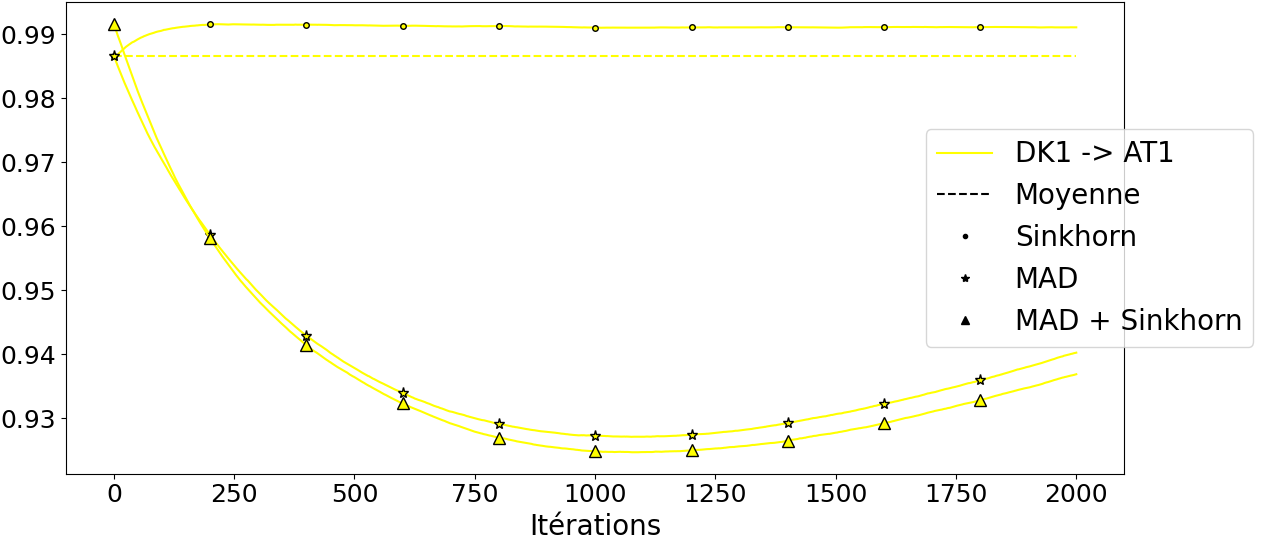
\includegraphics[scale=0.14]{images/50_biais_AT1.png}
        \caption{50\% de données manquantes}
        \label{50_biais_AT1}
    \end{subfigure}
    \hfill
    \begin{subfigure}[b]{0.4\textwidth}
        \raggedleft
        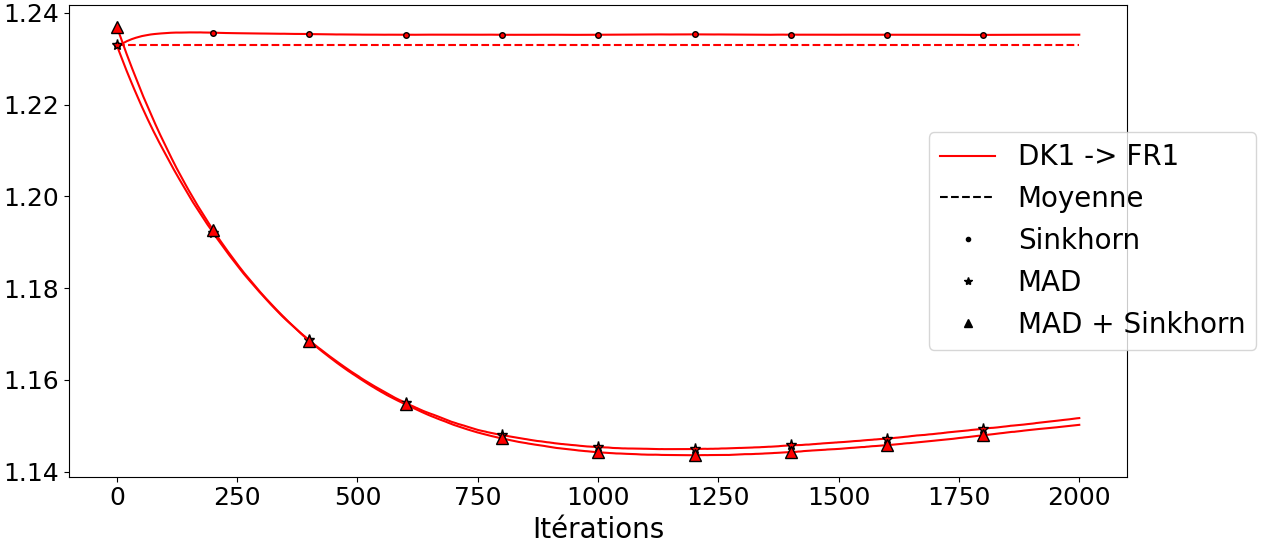
\includegraphics[scale=0.14]{images/90_biais_FR1.png}
        \caption{90\% de données manquantes}
        \label{90_biais_FR1}
    \end{subfigure}
       \caption{RMSE en fonction du nombre d'itérations}
\end{figure}

Mais ce n'est pas forcément le cas pour tous, par exemple:

\begin{figure}[H]
    \centering
    \begin{subfigure}[b]{0.4\textwidth}
        \centering
        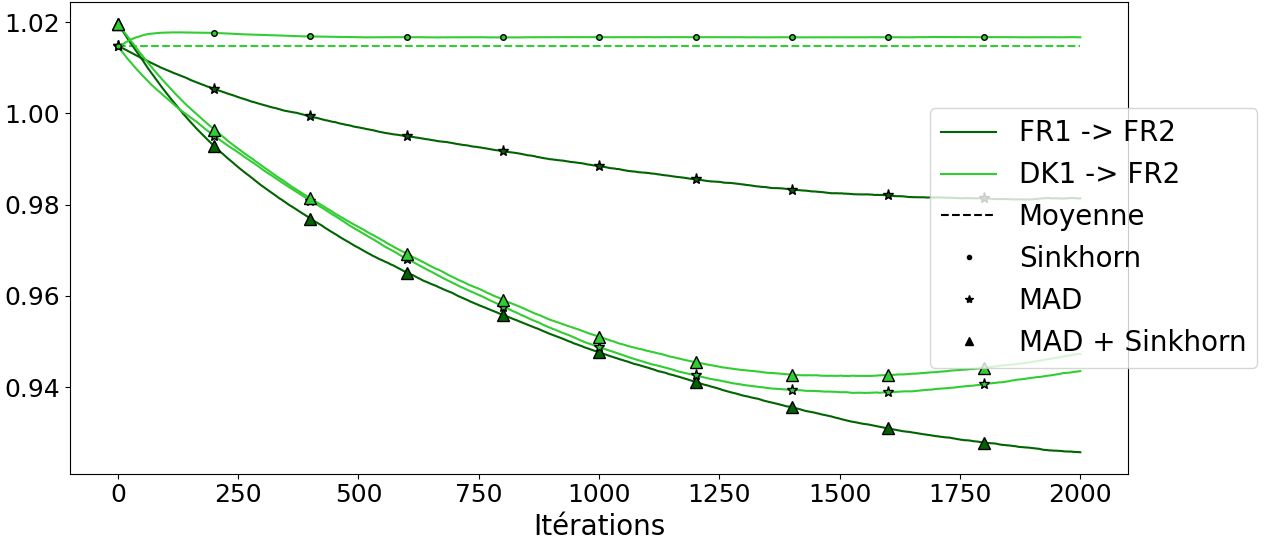
\includegraphics[scale=0.14]{images/50_biais_FR2.png}
        \caption{50\% de données manquantes}
        \label{50_biais_FR2}
    \end{subfigure}
    \hfill
    \begin{subfigure}[b]{0.4\textwidth}
        \centering
        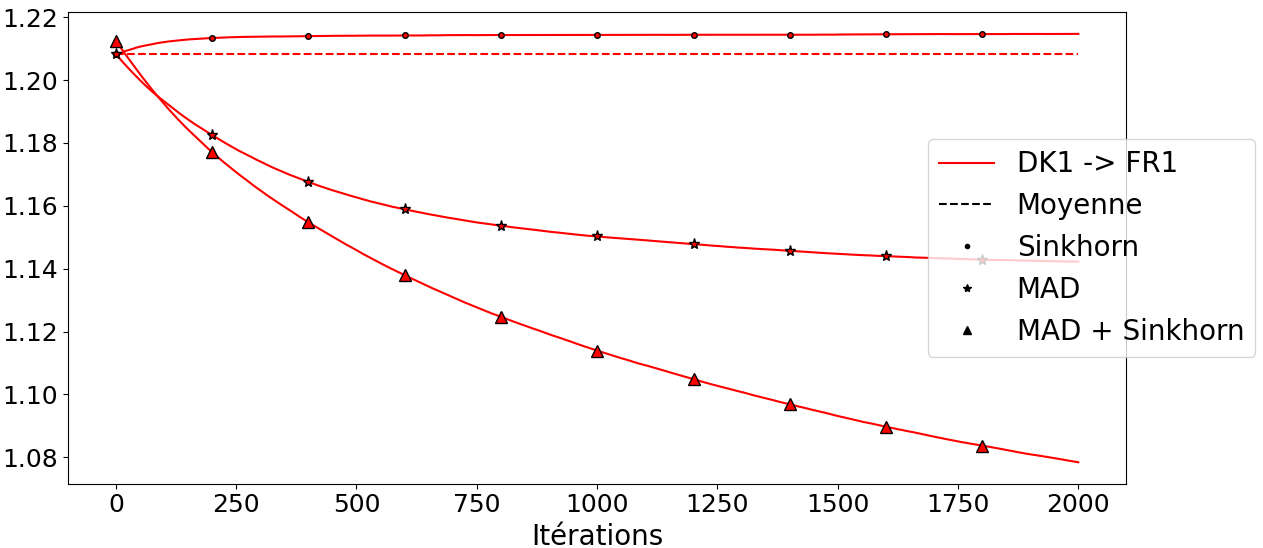
\includegraphics[scale=0.14]{images/60_biais_FR1.png}
        \caption{60\% de données manquantes}
        \label{60_biais_FR1}
    \end{subfigure}
    \hfill
    \begin{subfigure}[b]{0.4\textwidth}
        \centering
        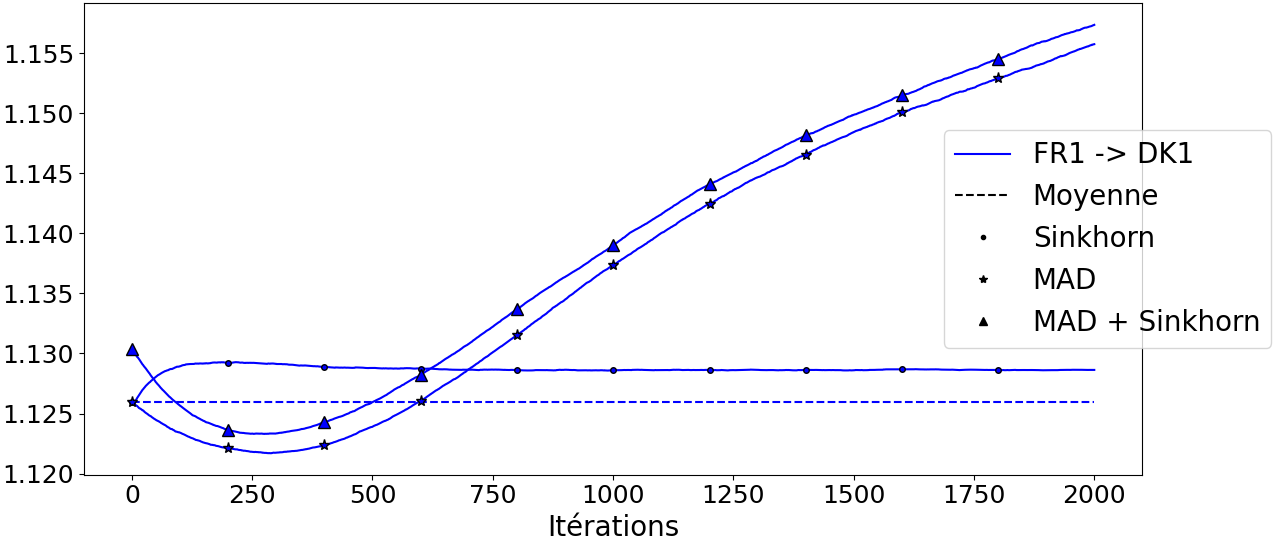
\includegraphics[scale=0.14]{images/60_biais_DK1.png}
        \caption{60\% de données manquantes}
        \label{60_biais_DK1}
    \end{subfigure}
    \hfill
    \begin{subfigure}[b]{0.4\textwidth}
        \centering
        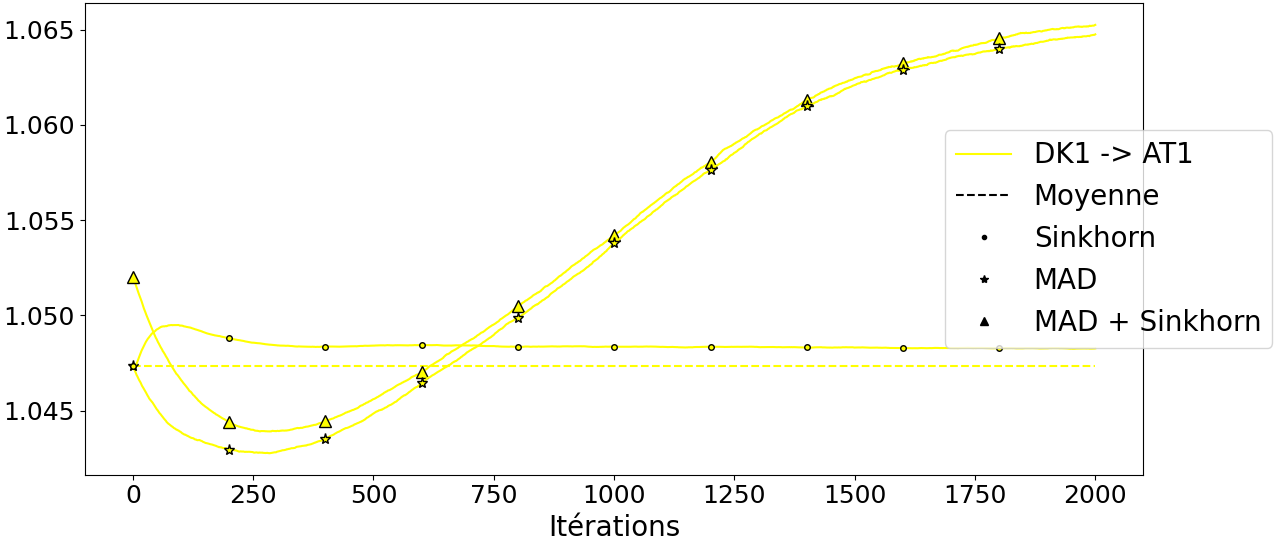
\includegraphics[scale=0.14]{images/90_biais_AT1.png}
        \caption{90\% de données manquantes}
        \label{90_biais_AT1}
    \end{subfigure}
       \caption{RMSE en fonction du nombre d'itérations}
\end{figure}

Dans les graphes de la figure~\ref{50_biais_FR2} et ~\ref{60_biais_FR1}, on remarque que la combinaison de MAD et Sinkhorn n'a pas atteint son minimum.
De plus, on peut avoir des cas de figures où la RMSE atteint un minimum plus bas que la moyenne, puis remonte au dessus de la moyenne avant les 1000 itérations,
comme pour la figure~\ref{60_biais_DK1} et ~\ref{90_biais_AT1}.
Ce qui pourrait inciter à faire un \textit{early stopping}.


\section{Conclusion}
Pour conclure, on observe que de façon générale, notre méthode a de meilleurs résultats que celle n'utilisant que le transport optimal.
Mais il peut arriver que l'on fasse pire après un trop grand nombre d'itérations, ce qui peut nous pousser à chercher à faire du \textit{early stopping},
pour estimer un nombre d'itérations raisonnable.
En outre, dans \textit{Missing Data Imputation using Optimal Transport}, il y a une autre méthode qui consiste à entrainer un réseau de neuronne pour faire la complétion de données,
en ayant toujours Sinkhorn pour fonction de coût, qui avait de meilleur résultat que l'imputation direct utilisé comme comparatif dans ce papier. 
On pourrait alors imaginer en faire de même en utilisant MAD comme fonction de coût.

\pagebreak
\begin{thebibliography}{99}


\bibitem[\protect\citeauthoryear{Muzellec}{2020}]{Muzellec2020}
[1] Muzellec, M., Josse, J., Boyer, C., Cuturi, M. Missing Data Imputation using Optimal Transport. 2020.

\bibitem[\protect\citeauthoryear{Cuturi}{2013}]{Cuturi2013}
[2] Cuturi, M. Sinkhorn distances: Lightspeed computation
of optimal transport. In \textit{Proceedings of the 26th International Conference on Neural Information Processing
Systems - Volume 2}, pp. 2292–2300, Red Hook, NY, USA,
2013. Curran Associates Inc.

\bibitem[\protect\citeauthoryear{Genevay}{2018}]{Genevay2018}
[3] Genevay, A., Peyre, G., and Cuturi, M. Learning generative models with Sinkhorn divergences. In Storkey, A. and Perez-Cruz, F. (eds.),
\textit{Proceedings of the Twenty-First International Conference on Artificial Intelligence and Statistics}, 
pp. 1608-1617, Playa Blanca, Lanzarote, Canary Islands, 09-11 Apr 2018. PMLR. 


\bibitem[\protect\citeauthoryear{Feydy}{2019}]{Feydy2019}
[4] Feydy, J., Séjourné, T., Vialard, F., Amari, S., Trouvé, A., and Peyré, G. Interpolationg between optimal transport and MMD using Sinkhorn divergences.
\textit{In The 22nd International Conference on Artificial Intelligence and Statistics,
AISTATS 2019, 16-18 April 2019, Naha, Okinawa, Japan,}
pp. 2681-2690, 2019.

\bibitem[\protect\citeauthoryear{Sakoe}{1978}]{Sakoe1978}
[5] Sakoe, H., Chiba, S.: Dynamic programming algorithm optimization for spoken
word recognition. IEEE transactions on acoustics, speech, and signal processing
26(1), 43–49 (1978)

\end{thebibliography}

\pagebreak
\section{Annexes}
\subsection{Manquantes au hasard}

\begin{figure}[H]
	\begin{minipage}[b]{0.4\linewidth}
		\centering 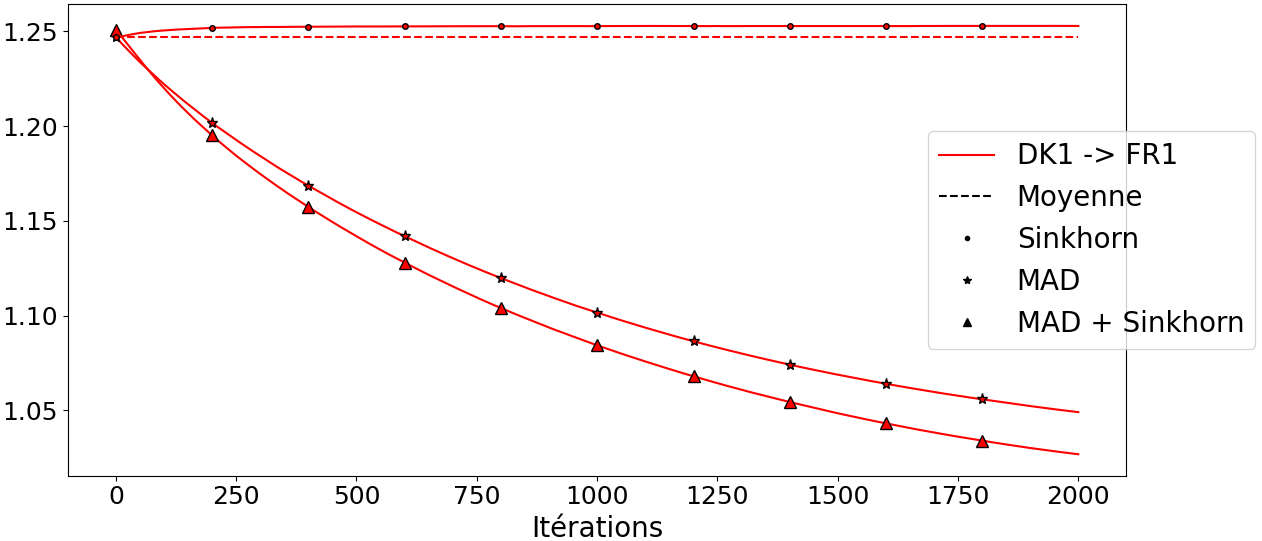
\includegraphics[scale=0.14]{images/50_ar_FR1.png}
		\caption{RMSE en fonction du nombre d'itération avec 50\% de données manquantes}
	\end{minipage}\hfill
    \begin{minipage}[b]{0.4\linewidth}
		\centering 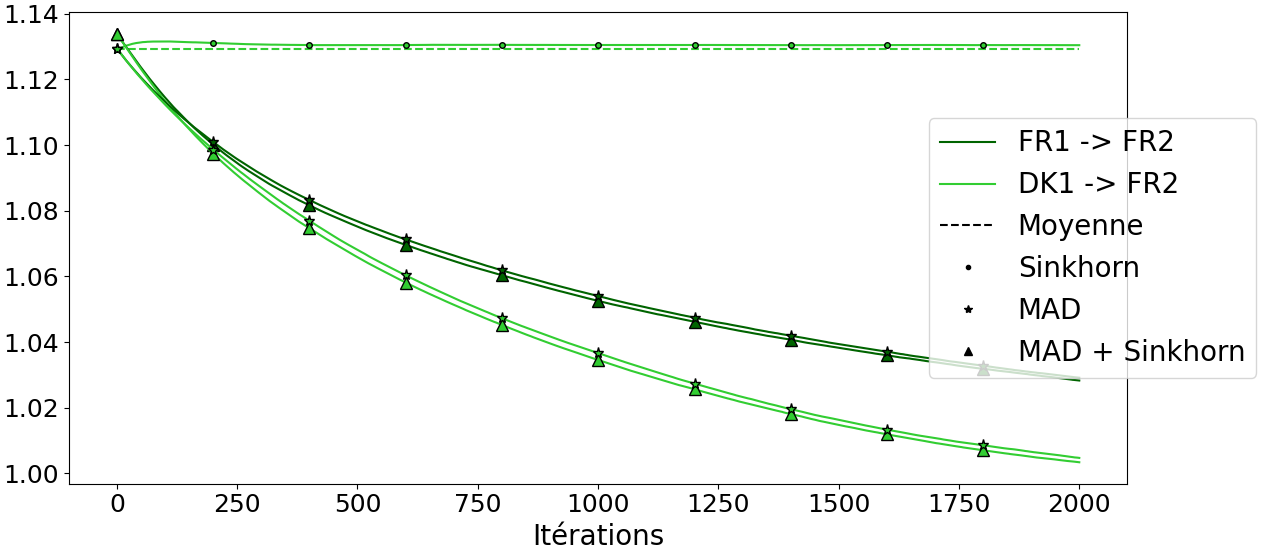
\includegraphics[scale=0.14]{images/50_ar_FR2.png}
		\caption{RMSE en fonction du nombre d'itération avec 50\% de données manquantes}
	\end{minipage}\hfill
    \begin{minipage}[b]{0.4\linewidth}
		\centering 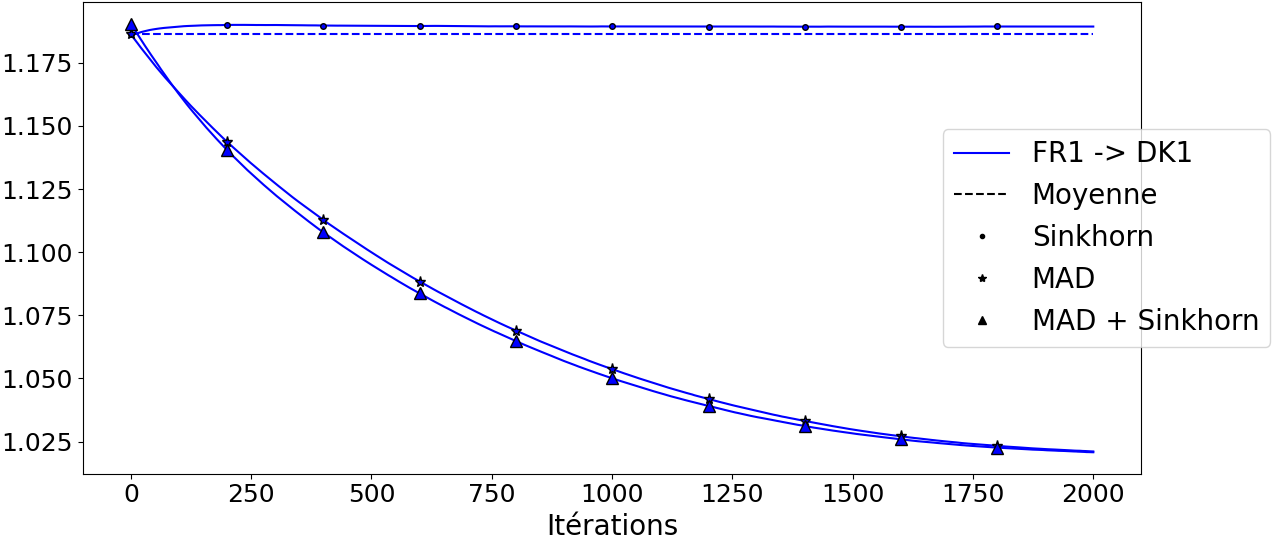
\includegraphics[scale=0.14]{images/50_ar_DK1.png}
		\caption{RMSE en fonction du nombre d'itération avec 50\% de données manquantes}
	\end{minipage}\hfill
    \begin{minipage}[b]{0.4\linewidth}
		\centering 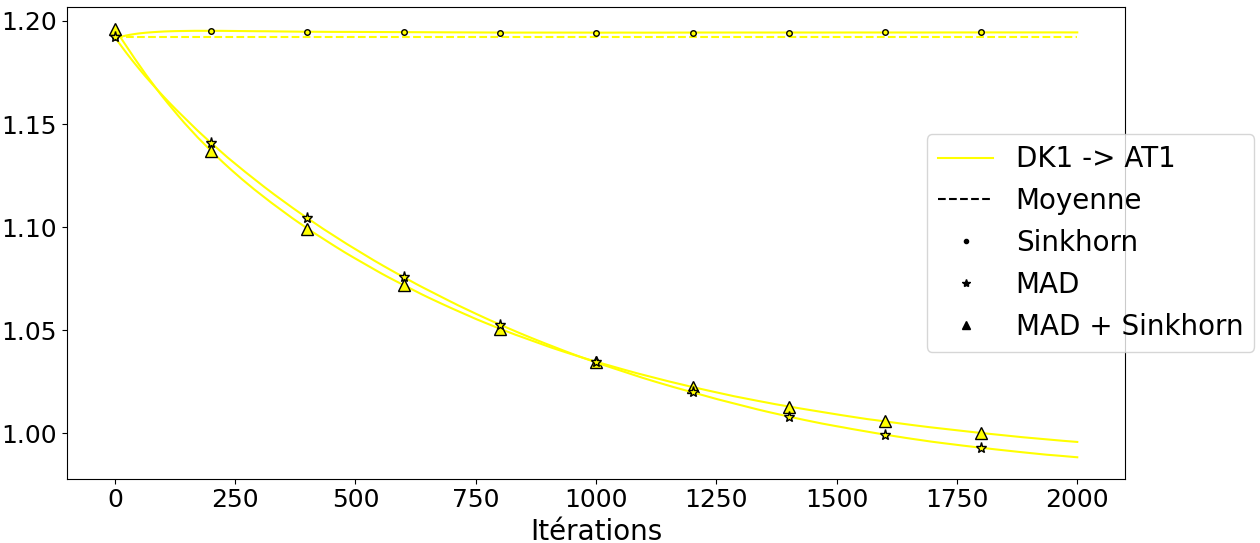
\includegraphics[scale=0.14]{images/50_ar_AT1.png}
		\caption{RMSE en fonction du nombre d'itération avec 50\% de données manquantes}
	\end{minipage}\hfill
    \begin{minipage}[b]{0.4\linewidth}
		\centering 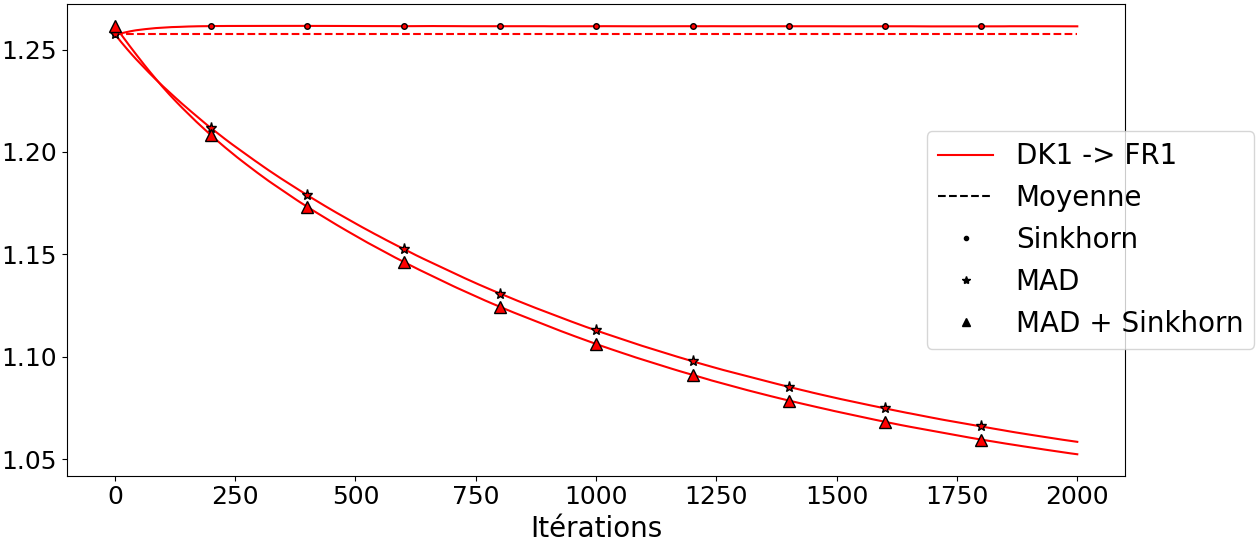
\includegraphics[scale=0.14]{images/60_ar_FR1.png}
		\caption{RMSE en fonction du nombre d'itération avec 60\% de données manquantes}
	\end{minipage}\hfill
    \begin{minipage}[b]{0.4\linewidth}
		\centering 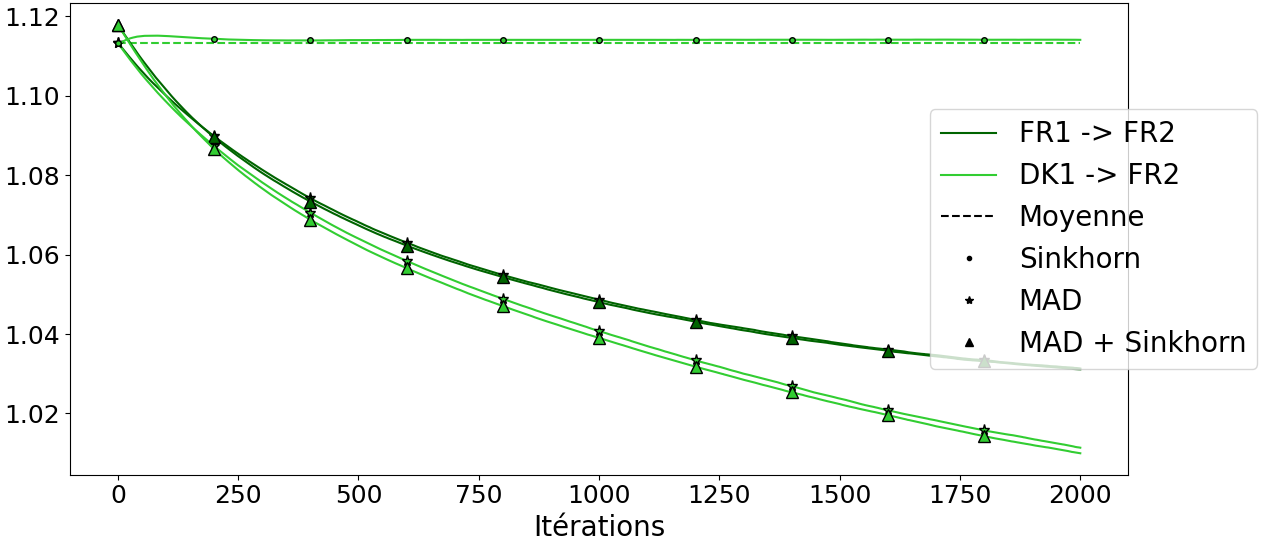
\includegraphics[scale=0.14]{images/60_ar_FR2.png}
		\caption{RMSE en fonction du nombre d'itération avec 60\% de données manquantes}
	\end{minipage}
\end{figure}
\begin{figure}[H]
    \begin{minipage}[b]{0.4\linewidth}
		\centering 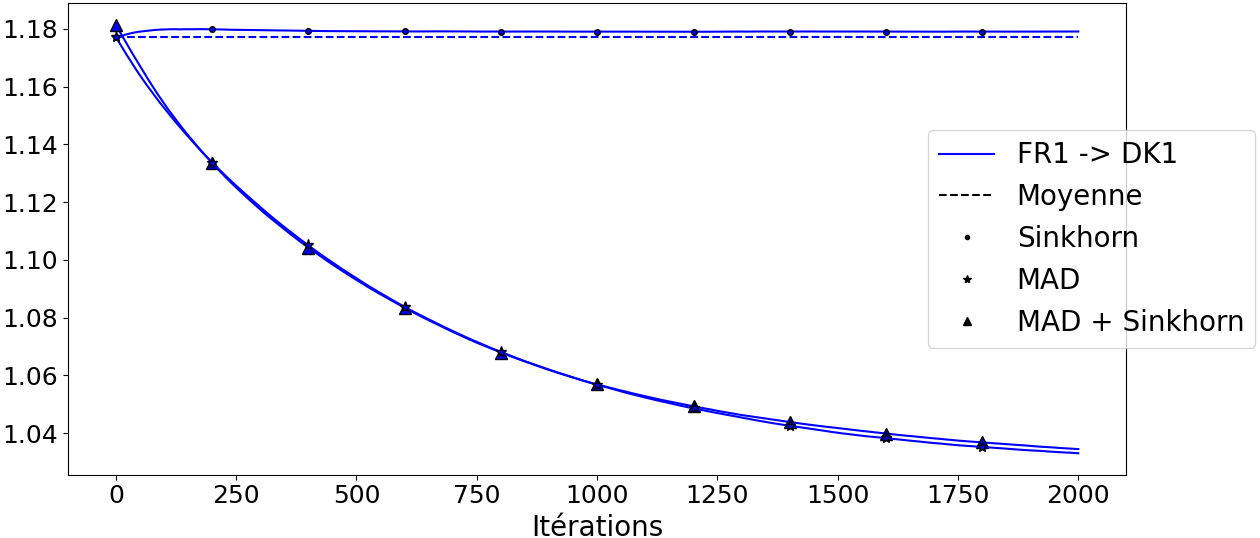
\includegraphics[scale=0.14]{images/60_ar_DK1.png}
		\caption{RMSE en fonction du nombre d'itération avec 60\% de données manquantes}
	\end{minipage}\hfill
    \begin{minipage}[b]{0.4\linewidth}
		\centering 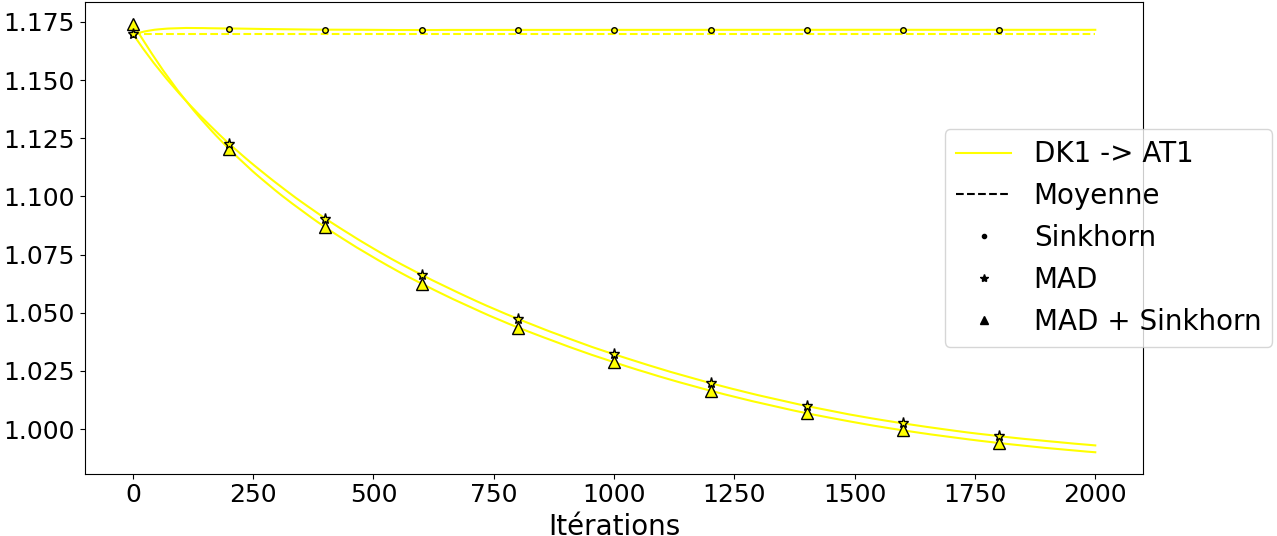
\includegraphics[scale=0.14]{images/60_ar_AT1.png}
		\caption{RMSE en fonction du nombre d'itération avec 60\% de données manquantes}
	\end{minipage}\hfill
    \begin{minipage}[b]{0.4\linewidth}
		\centering 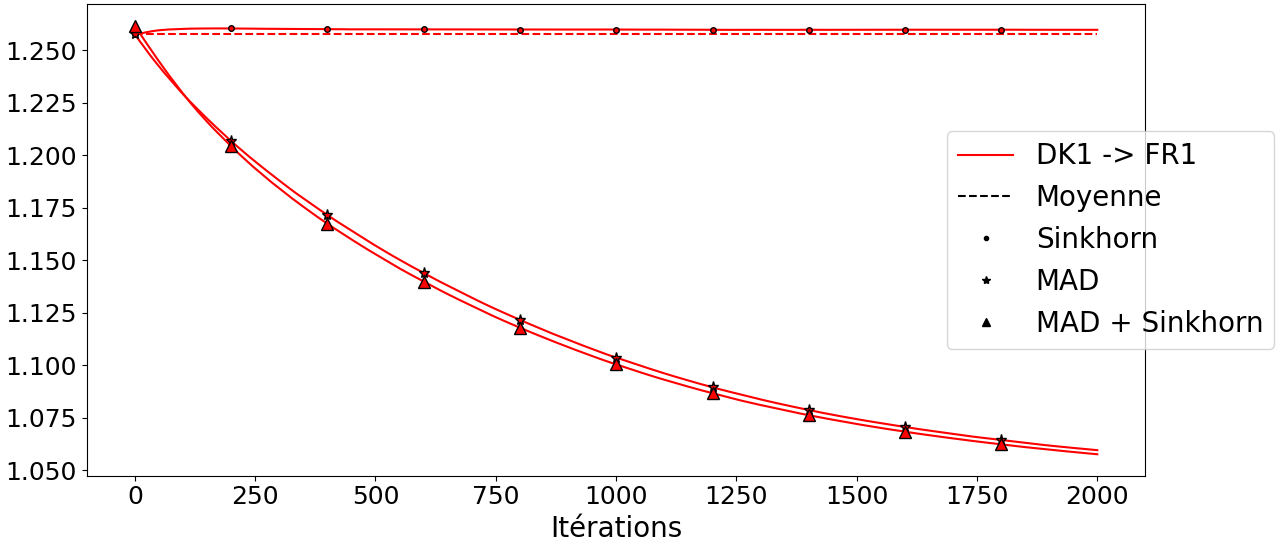
\includegraphics[scale=0.14]{images/70_ar_FR1.png}
		\caption{RMSE en fonction du nombre d'itération avec 70\% de données manquantes}
	\end{minipage}\hfill
    \begin{minipage}[b]{0.4\linewidth}
		\centering 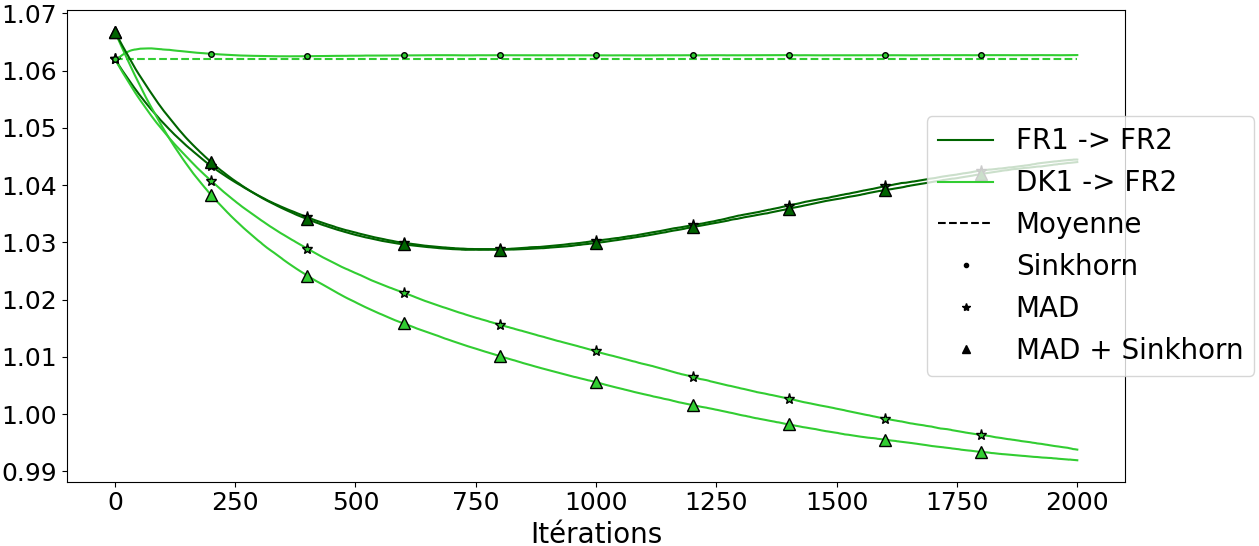
\includegraphics[scale=0.14]{images/70_ar_FR2.png}
		\caption{RMSE en fonction du nombre d'itération avec 70\% de données manquantes}
	\end{minipage}\hfill
    \begin{minipage}[b]{0.4\linewidth}
		\centering 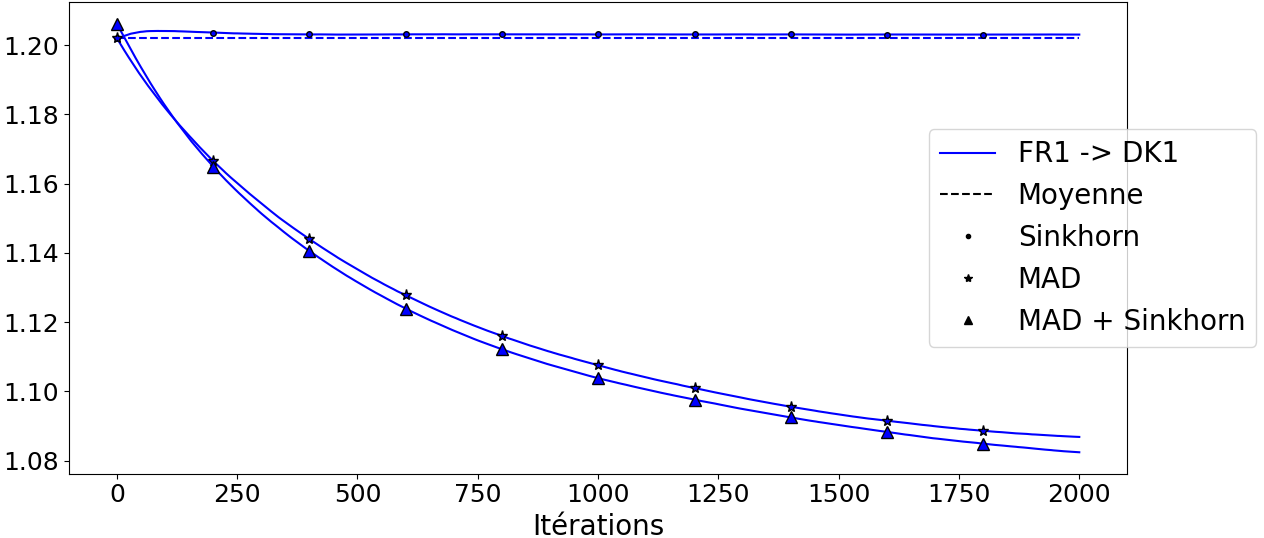
\includegraphics[scale=0.14]{images/70_ar_DK1.png}
		\caption{RMSE en fonction du nombre d'itération avec 70\% de données manquantes}
	\end{minipage}\hfill
    \begin{minipage}[b]{0.4\linewidth}
		\centering 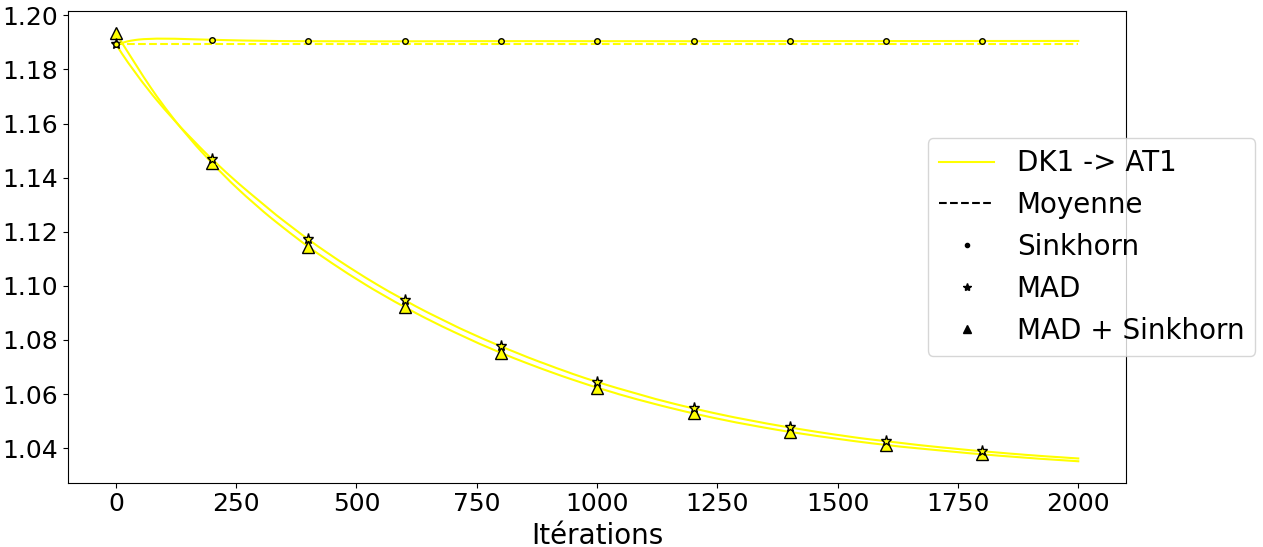
\includegraphics[scale=0.14]{images/70_ar_AT1.png}
		\caption{RMSE en fonction du nombre d'itération avec 70\% de données manquantes}
	\end{minipage}
\end{figure}
\begin{figure}[H]
    \begin{minipage}[b]{0.4\linewidth}
		\centering 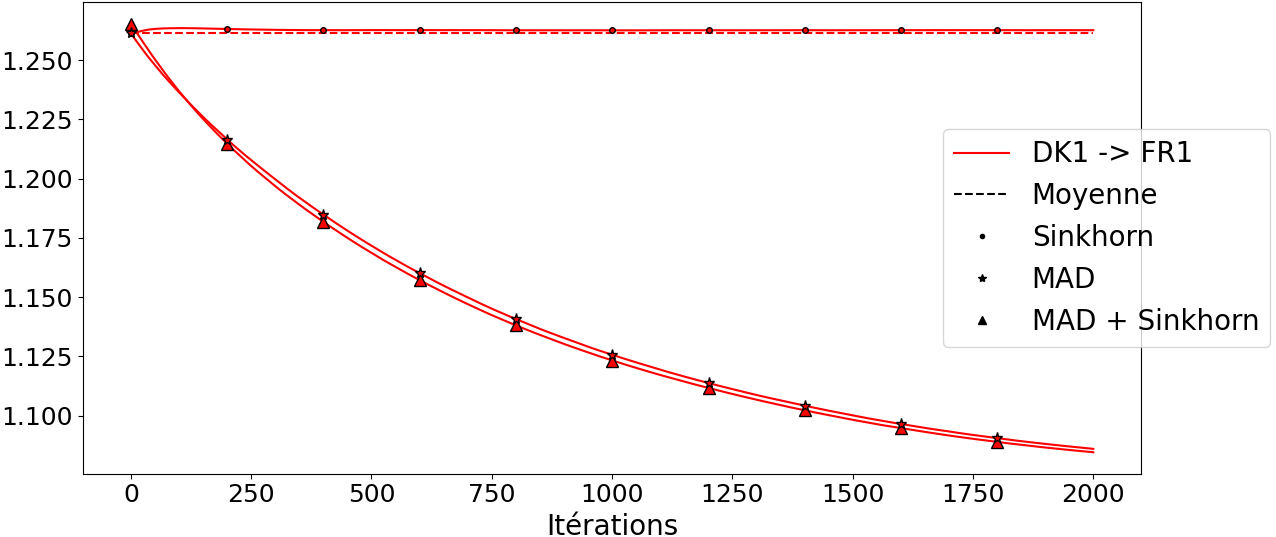
\includegraphics[scale=0.14]{images/80_ar_FR1.png}
		\caption{RMSE en fonction du nombre d'itération avec 80\% de données manquantes}
	\end{minipage}\hfill
    \begin{minipage}[b]{0.4\linewidth}
		\centering 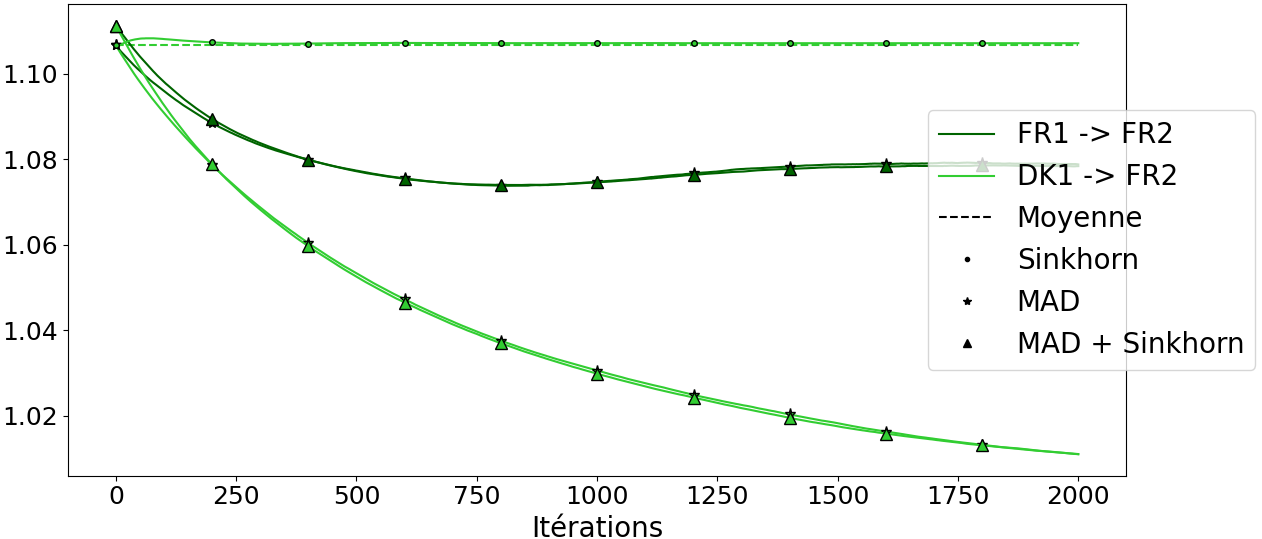
\includegraphics[scale=0.14]{images/80_ar_FR2.png}
		\caption{RMSE en fonction du nombre d'itération avec 80\% de données manquantes}
	\end{minipage}\hfill
    \begin{minipage}[b]{0.4\linewidth}
		\centering 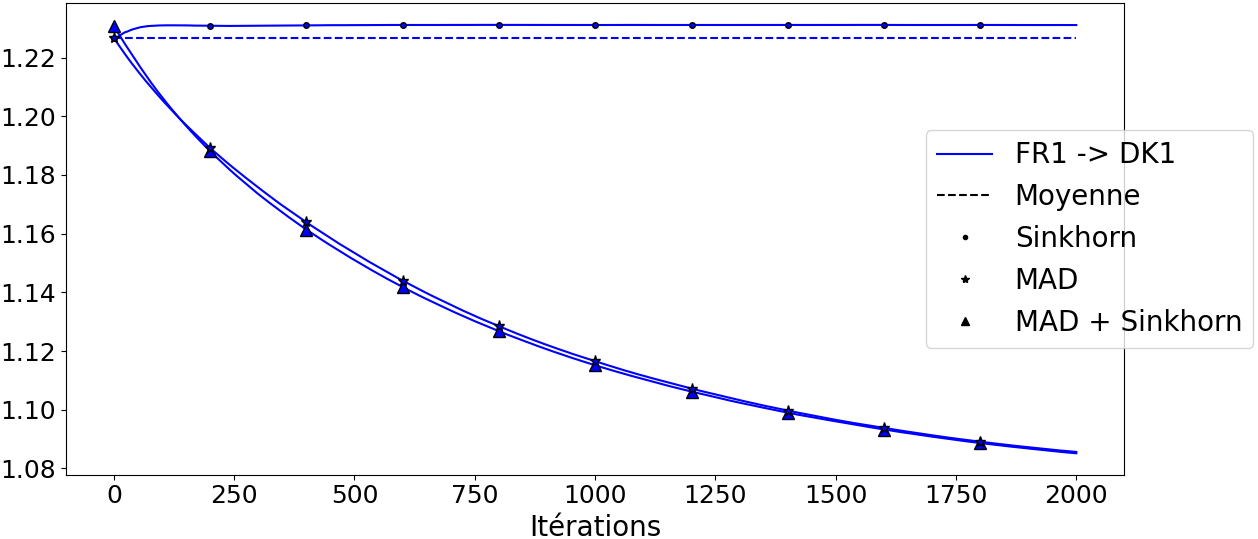
\includegraphics[scale=0.14]{images/80_ar_DK1.png}
		\caption{RMSE en fonction du nombre d'itération avec 80\% de données manquantes}
	\end{minipage}\hfill
    \begin{minipage}[b]{0.4\linewidth}
		\centering 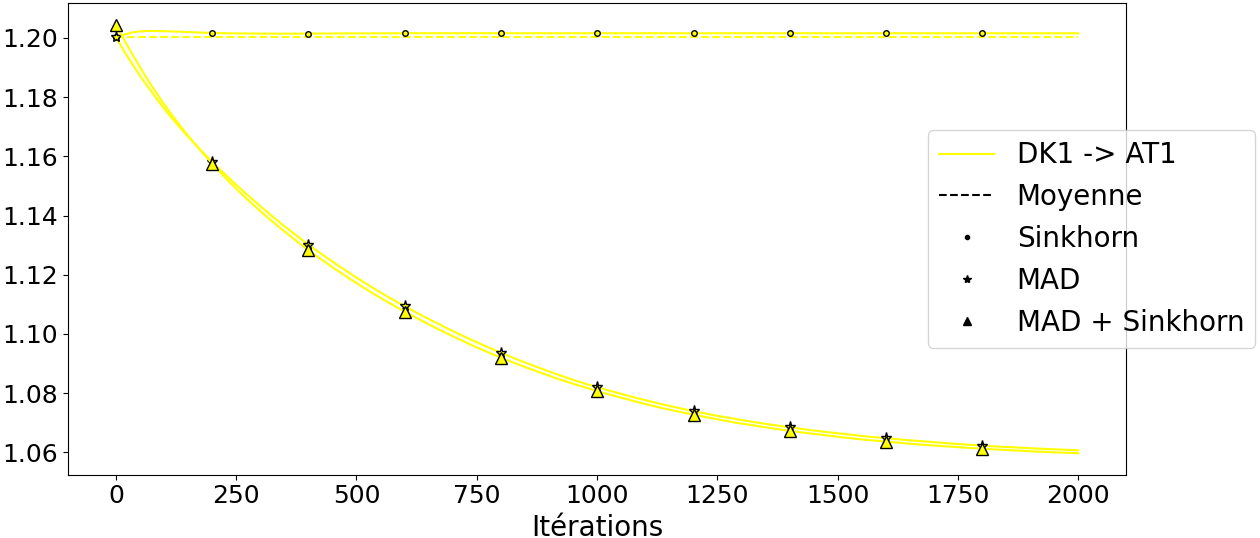
\includegraphics[scale=0.14]{images/80_ar_AT1.png}
		\caption{RMSE en fonction du nombre d'itération avec 80\% de données manquantes}
	\end{minipage}\hfill
    \begin{minipage}[b]{0.4\linewidth}
		\centering 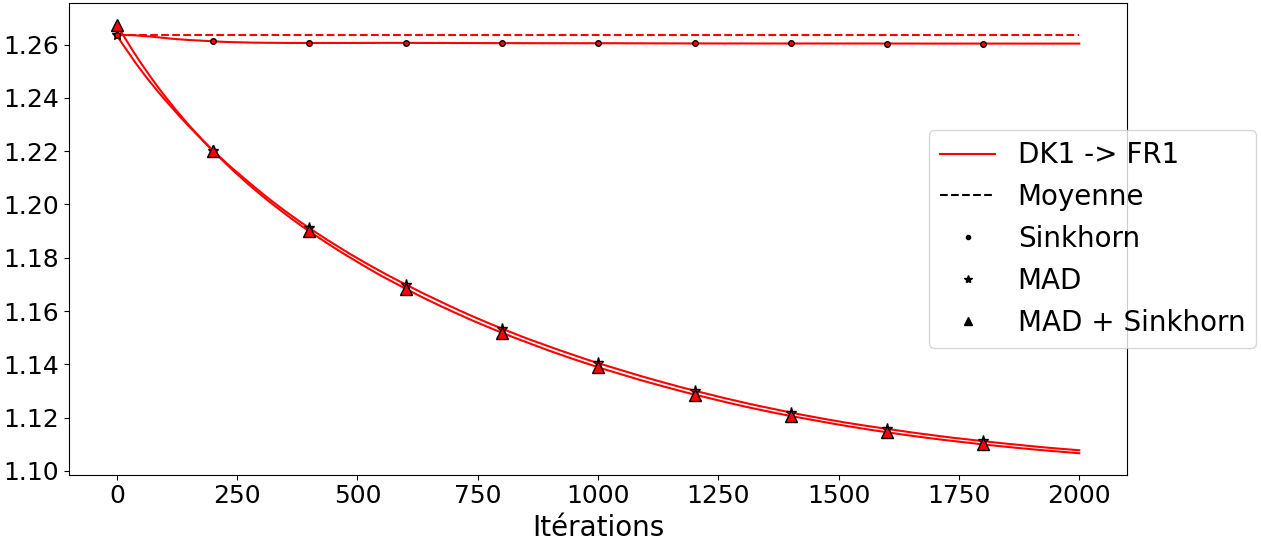
\includegraphics[scale=0.14]{images/90_ar_FR1.png}
		\caption{RMSE en fonction du nombre d'itération avec 90\% de données manquantes}
	\end{minipage}\hfill
    \begin{minipage}[b]{0.4\linewidth}
		\centering 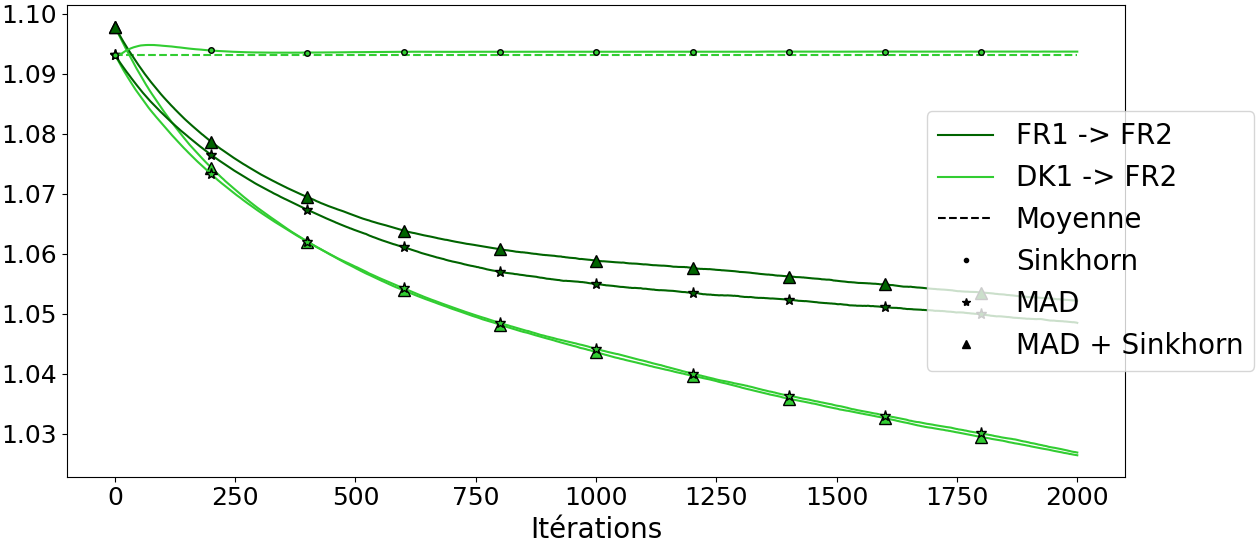
\includegraphics[scale=0.14]{images/90_ar_FR2.png}
		\caption{RMSE en fonction du nombre d'itération avec 90\% de données manquantes}
	\end{minipage}
\end{figure}
\begin{figure}[H]
    \begin{minipage}[b]{0.4\linewidth}
		\centering 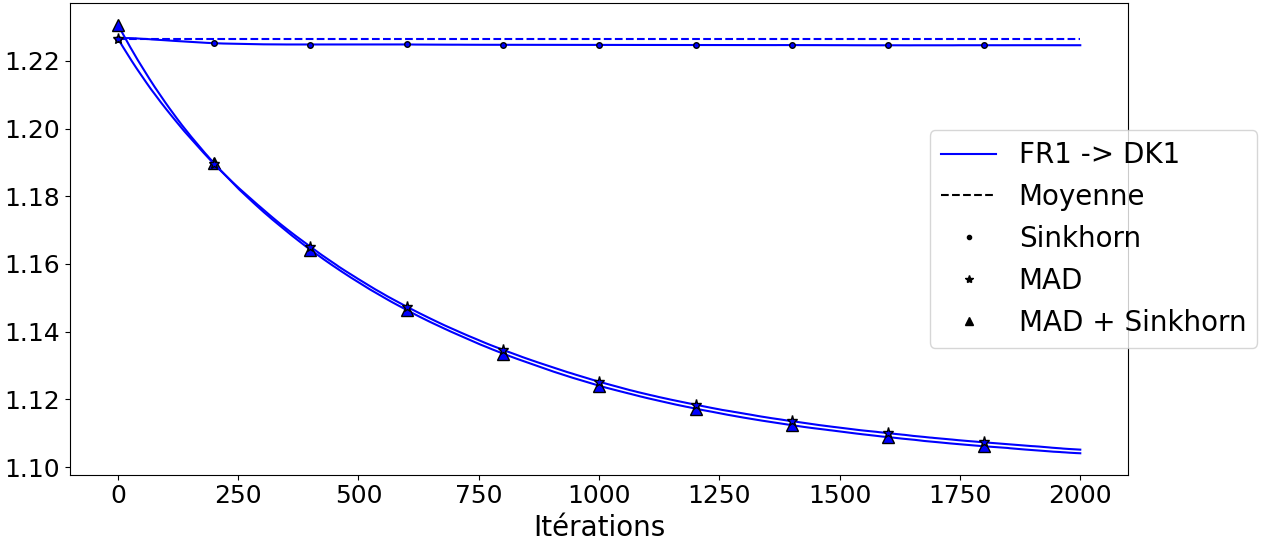
\includegraphics[scale=0.14]{images/90_ar_DK1.png}
		\caption{RMSE en fonction du nombre d'itération avec 90\% de données manquantes}
	\end{minipage}\hfill
	\begin{minipage}[b]{0.4\linewidth}	
		\centering 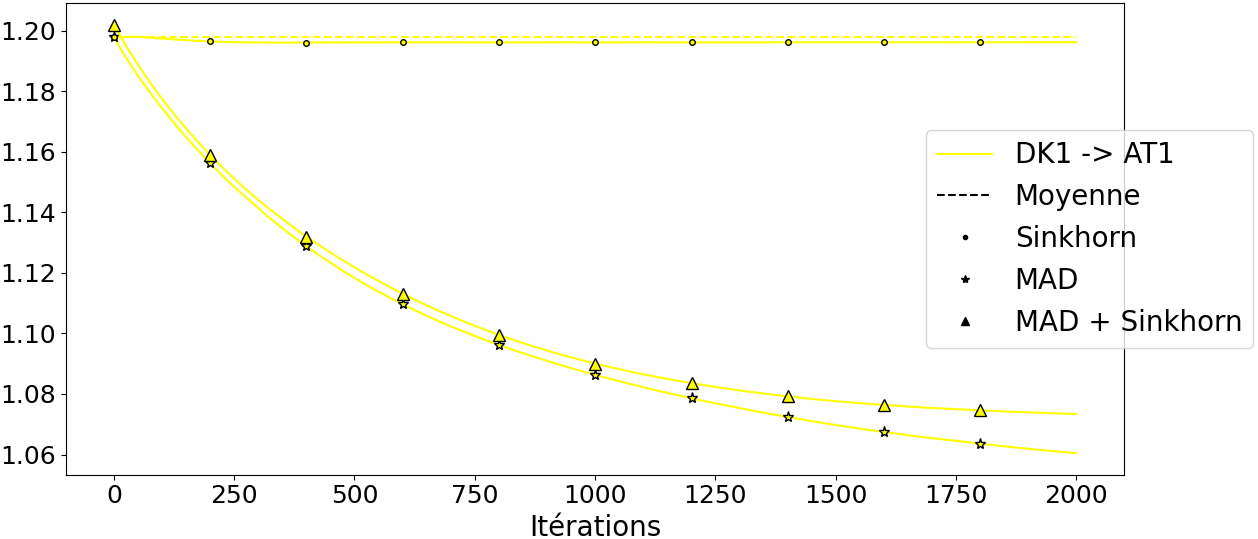
\includegraphics[scale=0.14]{images/90_ar_AT1.png}
		\caption{RMSE en fonction du nombre d'itération avec 90\% de données manquantes}
	\end{minipage}
\end{figure}

\subsection{Manquantes avec un biais}

\begin{figure}[H]
	\begin{minipage}[b]{0.4\linewidth}
		\centering 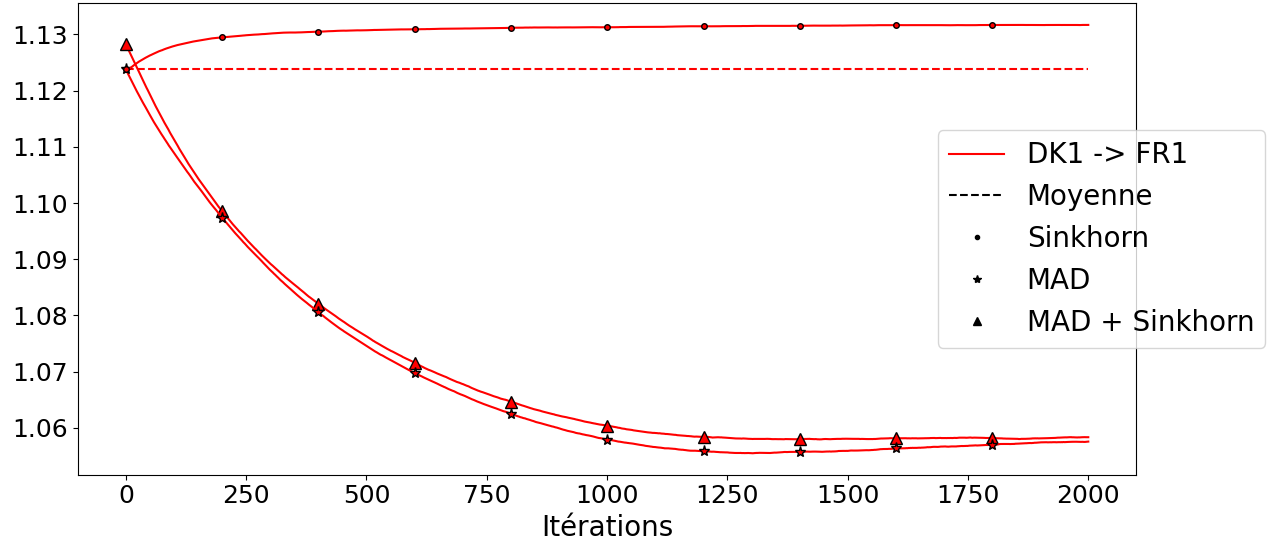
\includegraphics[scale=0.14]{images/50_biais_FR1.png}
		\caption{RMSE en fonction du nombre d'itération avec 50\% de données manquantes}
	\end{minipage}\hfill
    \begin{minipage}[b]{0.4\linewidth}
		\centering 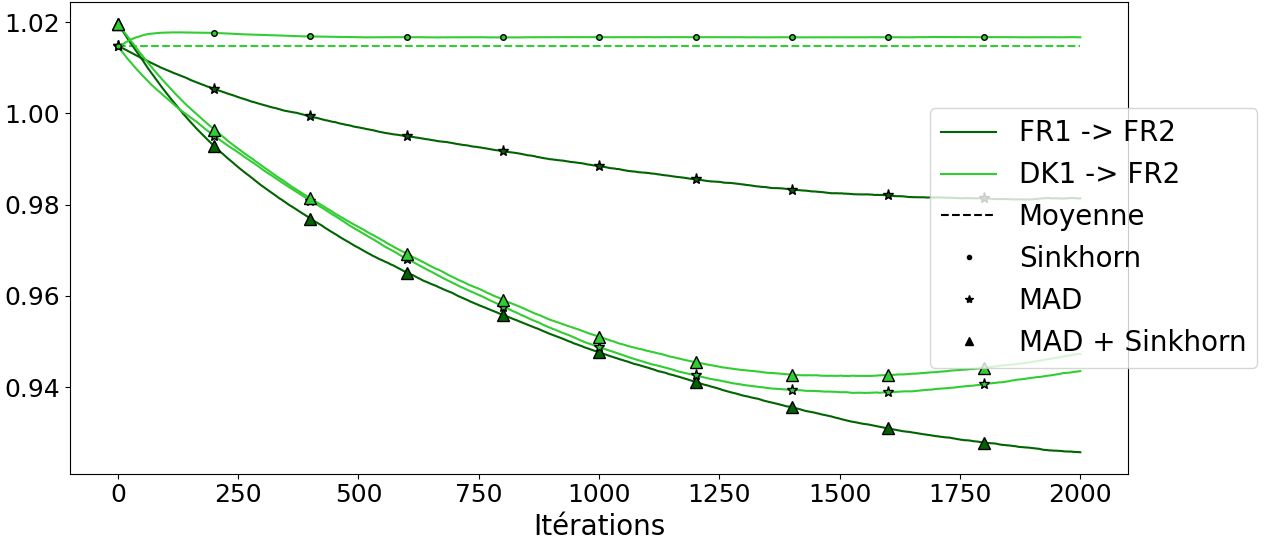
\includegraphics[scale=0.14]{images/50_biais_FR2.png}
		\caption{RMSE en fonction du nombre d'itération avec 50\% de données manquantes}
	\end{minipage}\hfill
    \begin{minipage}[b]{0.4\linewidth}
		\centering 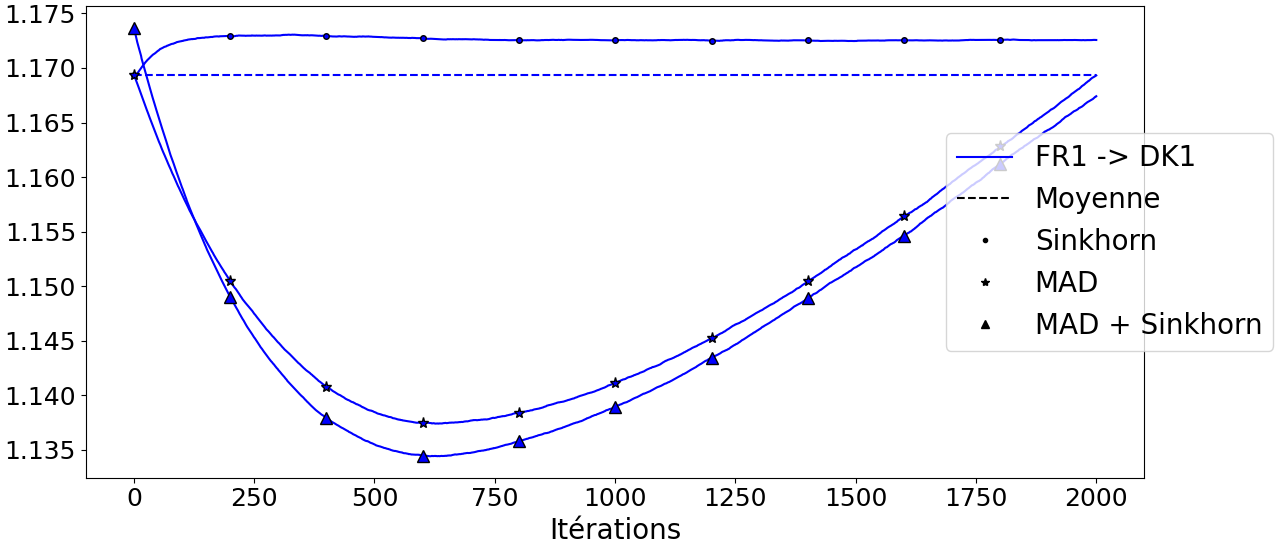
\includegraphics[scale=0.14]{images/50_biais_DK1.png}
		\caption{RMSE en fonction du nombre d'itération avec 50\% de données manquantes}
	\end{minipage}\hfill
    \begin{minipage}[b]{0.4\linewidth}
		\centering 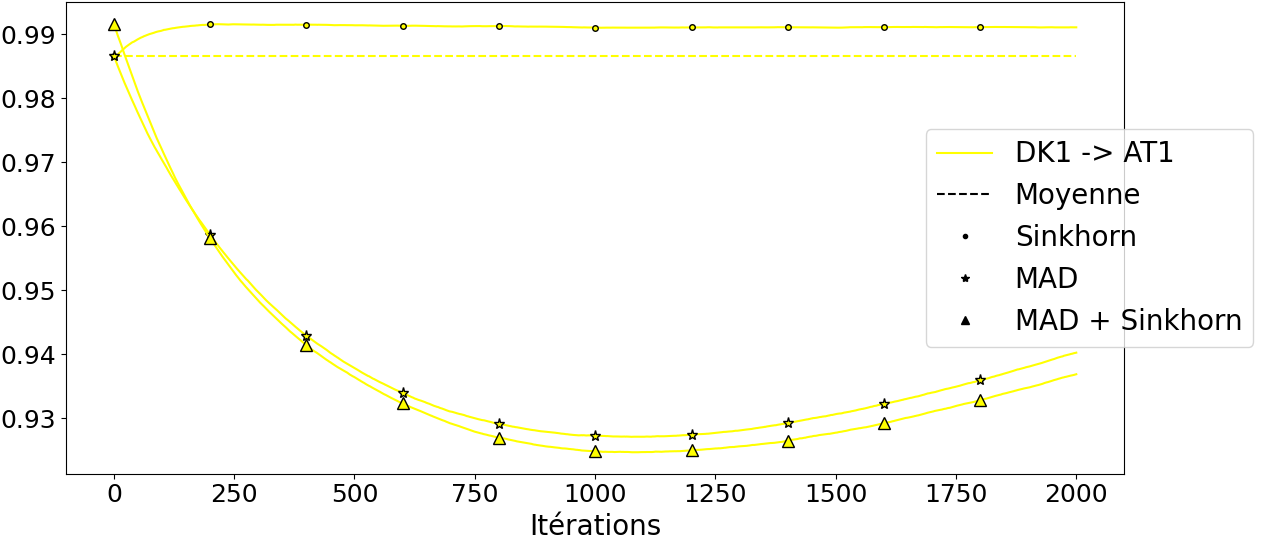
\includegraphics[scale=0.14]{images/50_biais_AT1.png}
		\caption{RMSE en fonction du nombre d'itération avec 50\% de données manquantes}
	\end{minipage}\hfill
    \begin{minipage}[b]{0.4\linewidth}
		\centering 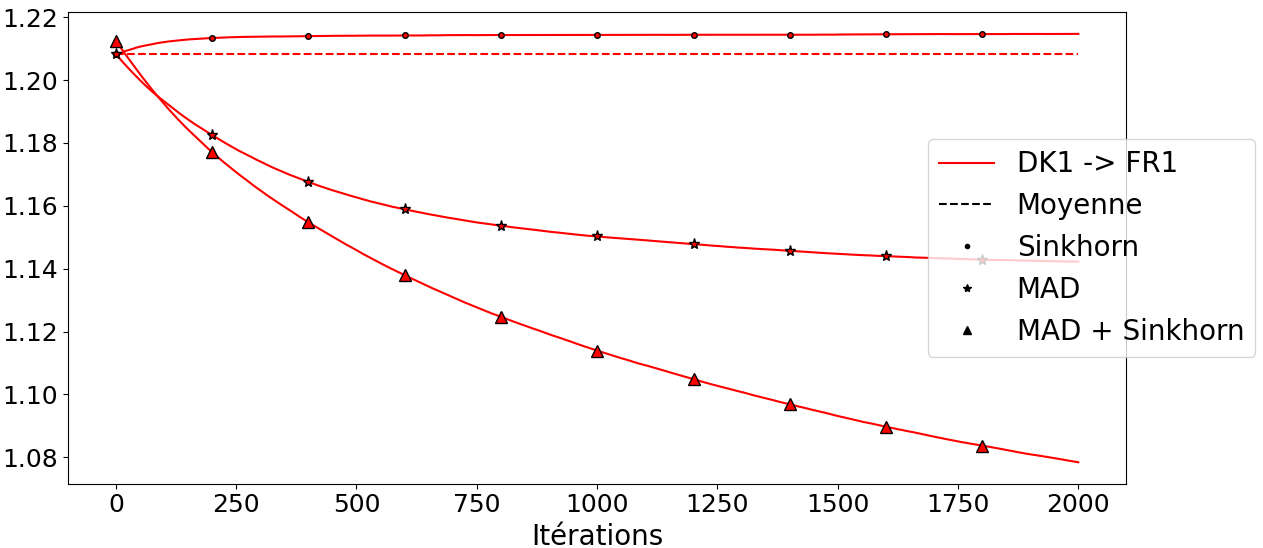
\includegraphics[scale=0.14]{images/60_biais_FR1.png}
		\caption{RMSE en fonction du nombre d'itération avec 60\% de données manquantes}
	\end{minipage}\hfill
    \begin{minipage}[b]{0.4\linewidth}
		\centering 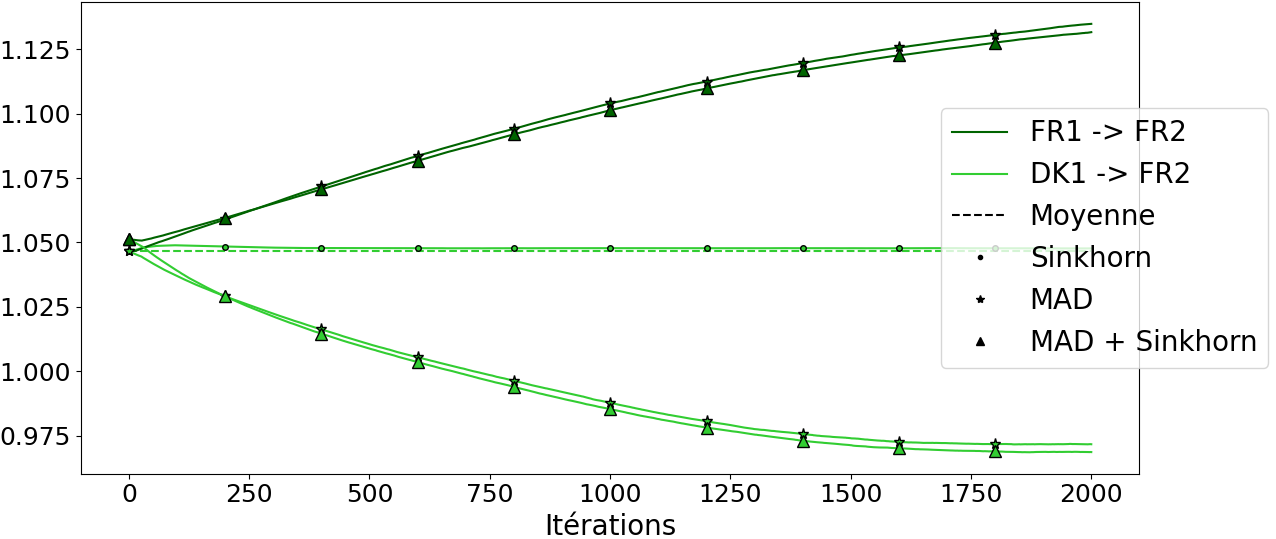
\includegraphics[scale=0.14]{images/60_biais_FR2.png}
		\caption{RMSE en fonction du nombre d'itération avec 60\% de données manquantes}
	\end{minipage}
\end{figure}
\begin{figure}[H]
    \begin{minipage}[b]{0.4\linewidth}
		\centering 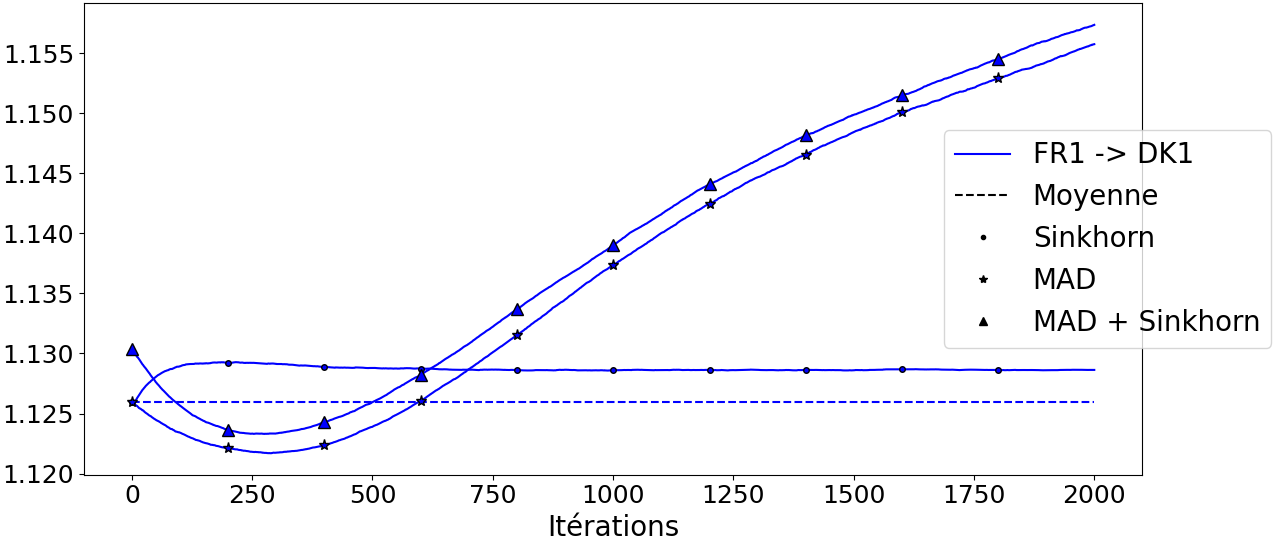
\includegraphics[scale=0.14]{images/60_biais_DK1.png}
		\caption{RMSE en fonction du nombre d'itération avec 60\% de données manquantes}
	\end{minipage}\hfill
    \begin{minipage}[b]{0.4\linewidth}
		\centering 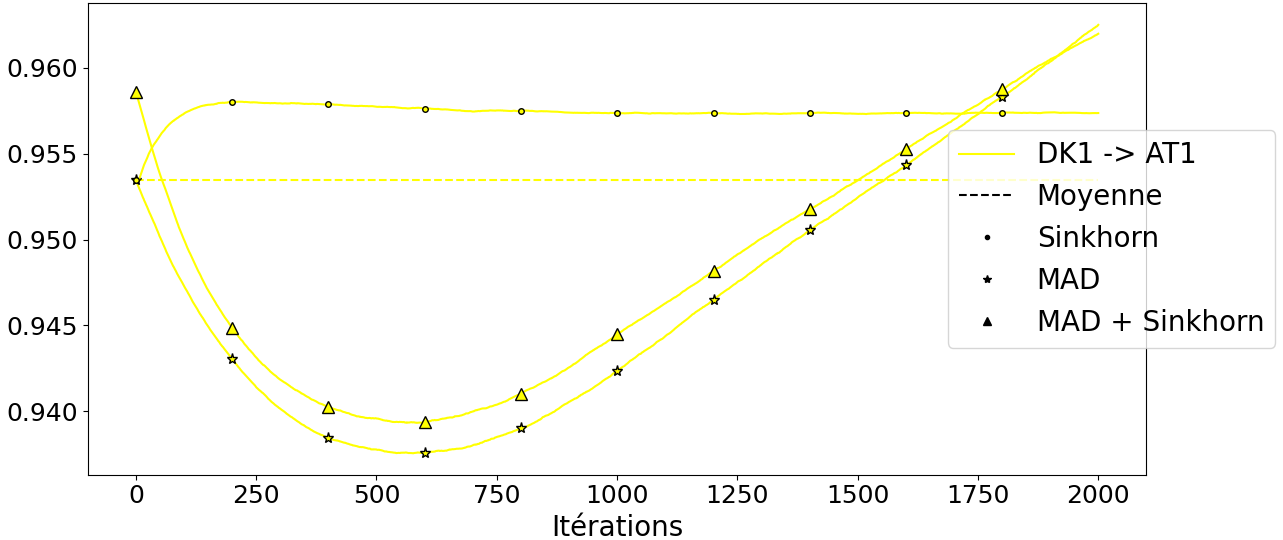
\includegraphics[scale=0.14]{images/60_biais_AT1.png}
		\caption{RMSE en fonction du nombre d'itération avec 60\% de données manquantes}
	\end{minipage}\hfill
    \begin{minipage}[b]{0.4\linewidth}
		\centering 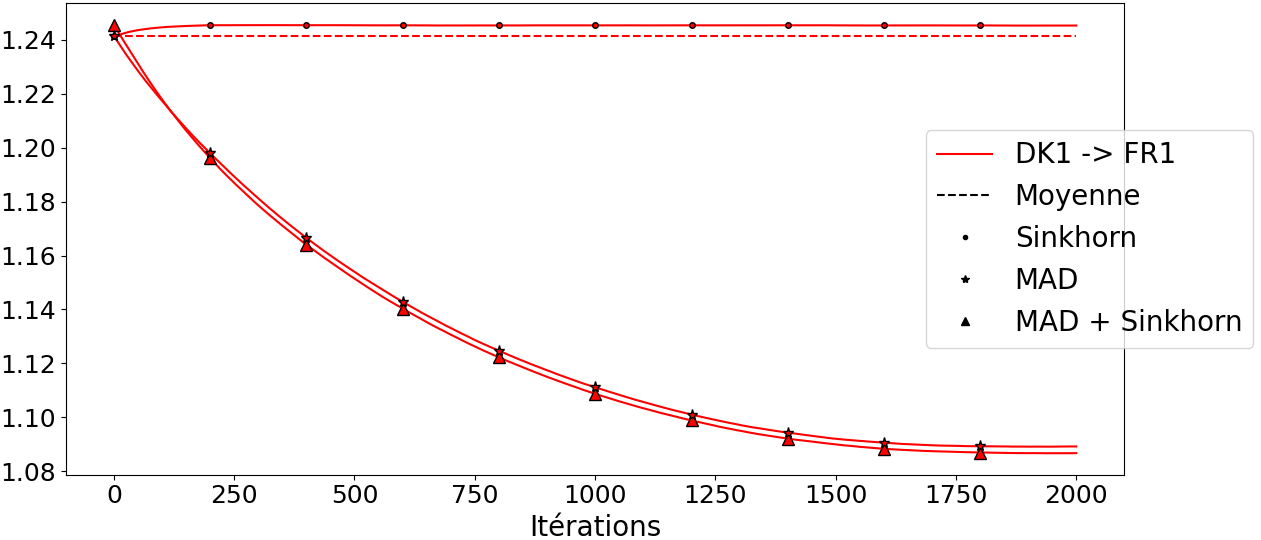
\includegraphics[scale=0.14]{images/70_biais_FR1.png}
		\caption{RMSE en fonction du nombre d'itération avec 70\% de données manquantes}
	\end{minipage}\hfill
    \begin{minipage}[b]{0.4\linewidth}
		\centering 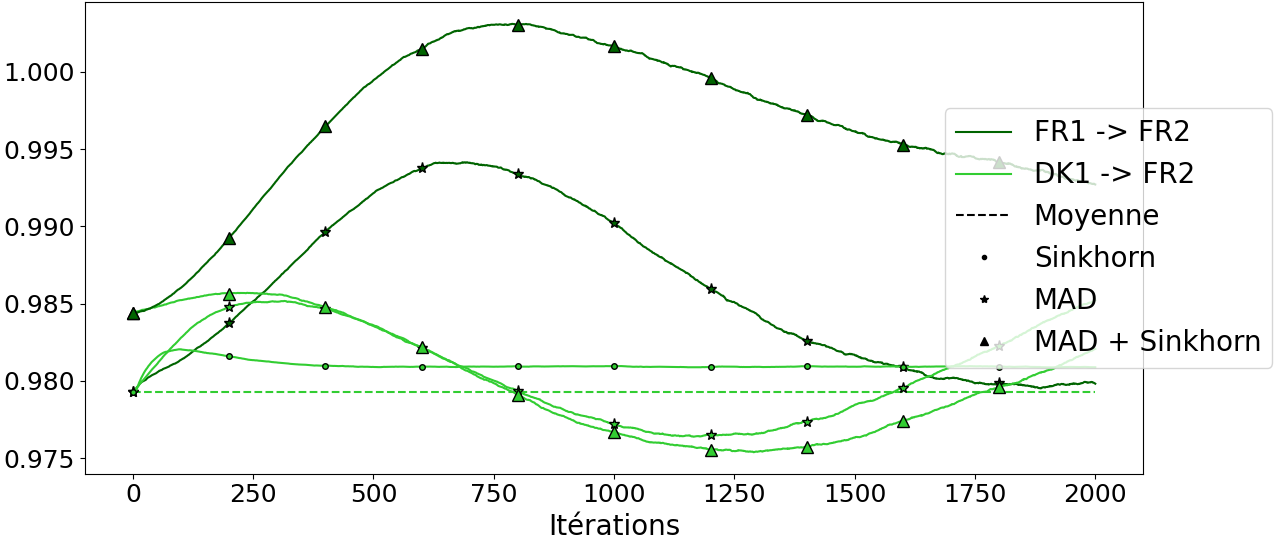
\includegraphics[scale=0.14]{images/70_biais_FR2.png}
		\caption{RMSE en fonction du nombre d'itération avec 70\% de données manquantes}
	\end{minipage}\hfill
    \begin{minipage}[b]{0.4\linewidth}
		\centering 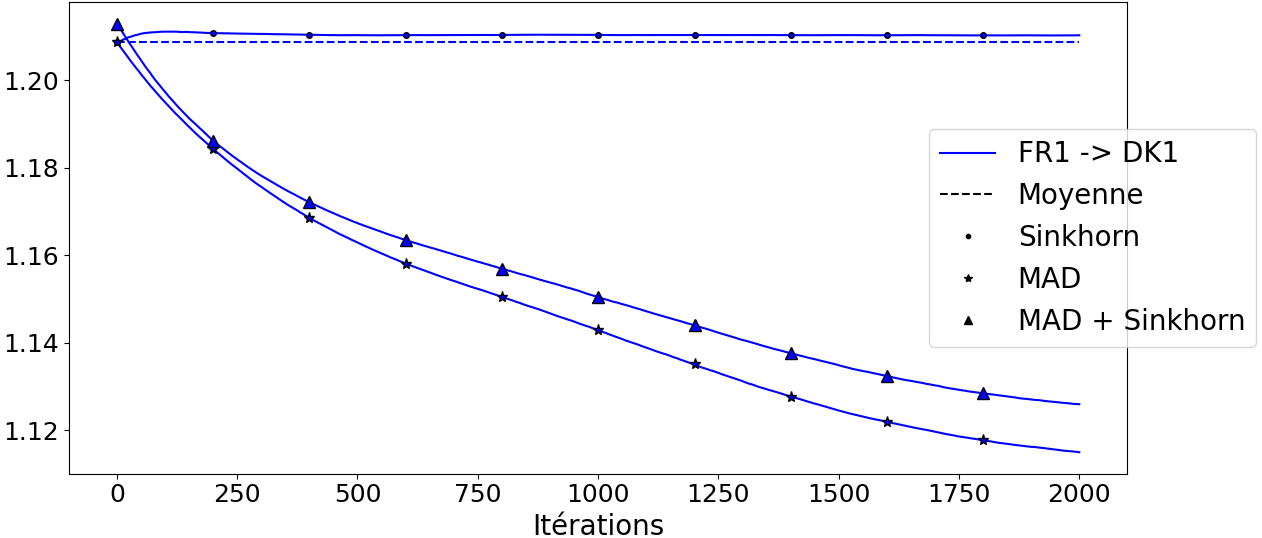
\includegraphics[scale=0.14]{images/70_biais_DK1.png}
		\caption{RMSE en fonction du nombre d'itération avec 70\% de données manquantes}
	\end{minipage}\hfill
    \begin{minipage}[b]{0.4\linewidth}
		\centering 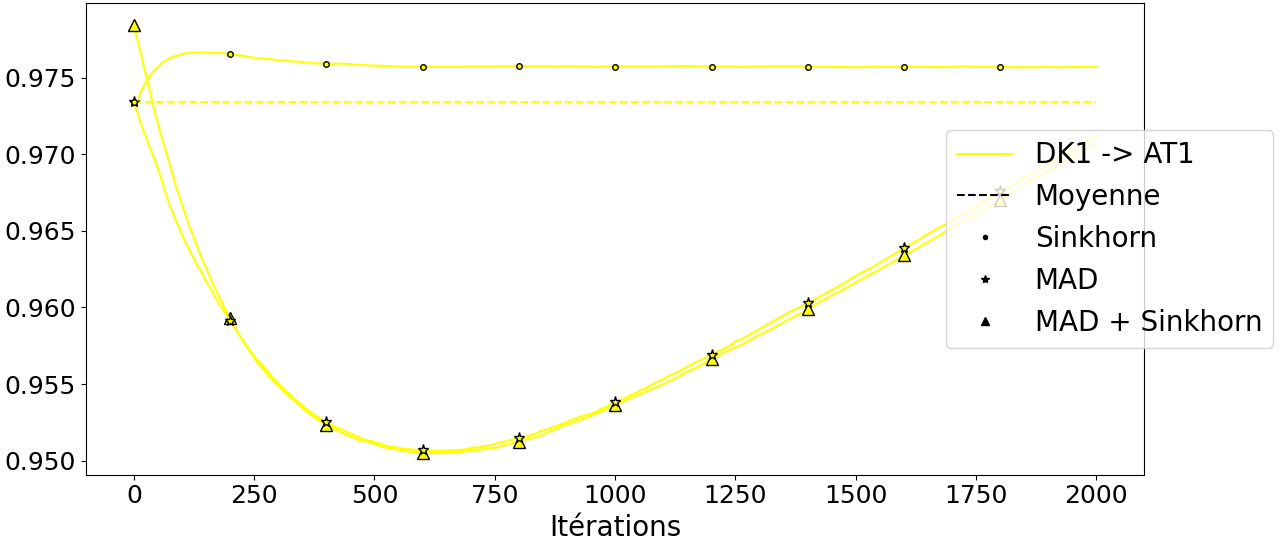
\includegraphics[scale=0.14]{images/70_biais_AT1.png}
		\caption{RMSE en fonction du nombre d'itération avec 70\% de données manquantes}
	\end{minipage}
\end{figure}
\begin{figure}[H]
    \begin{minipage}[b]{0.4\linewidth}
		\centering 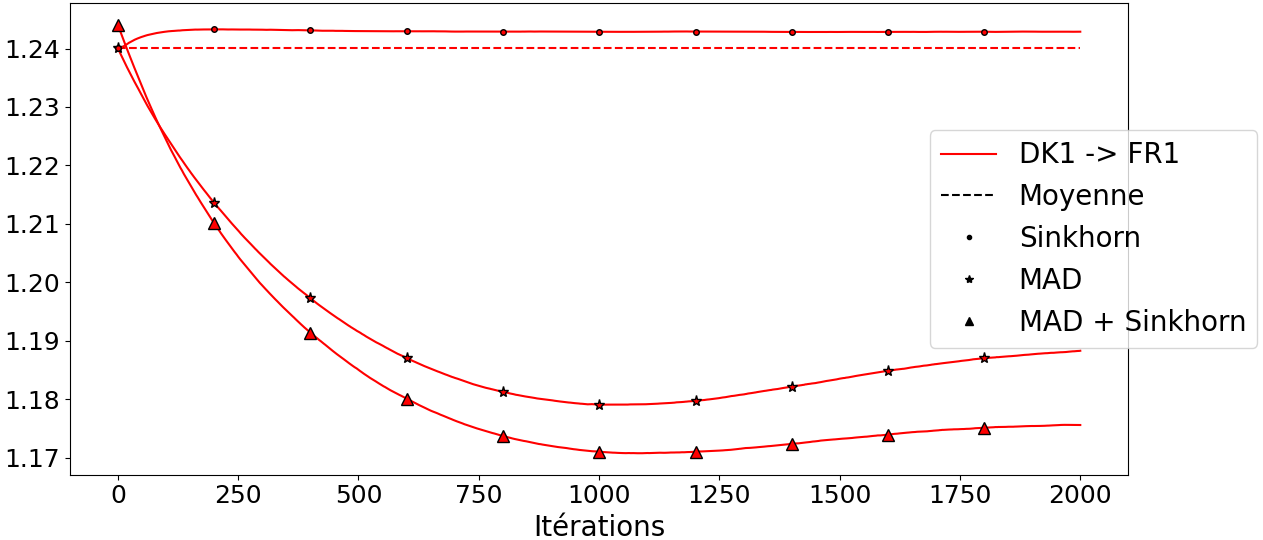
\includegraphics[scale=0.14]{images/80_biais_FR1.png}
		\caption{RMSE en fonction du nombre d'itération avec 80\% de données manquantes}
	\end{minipage}\hfill
    \begin{minipage}[b]{0.4\linewidth}
		\centering 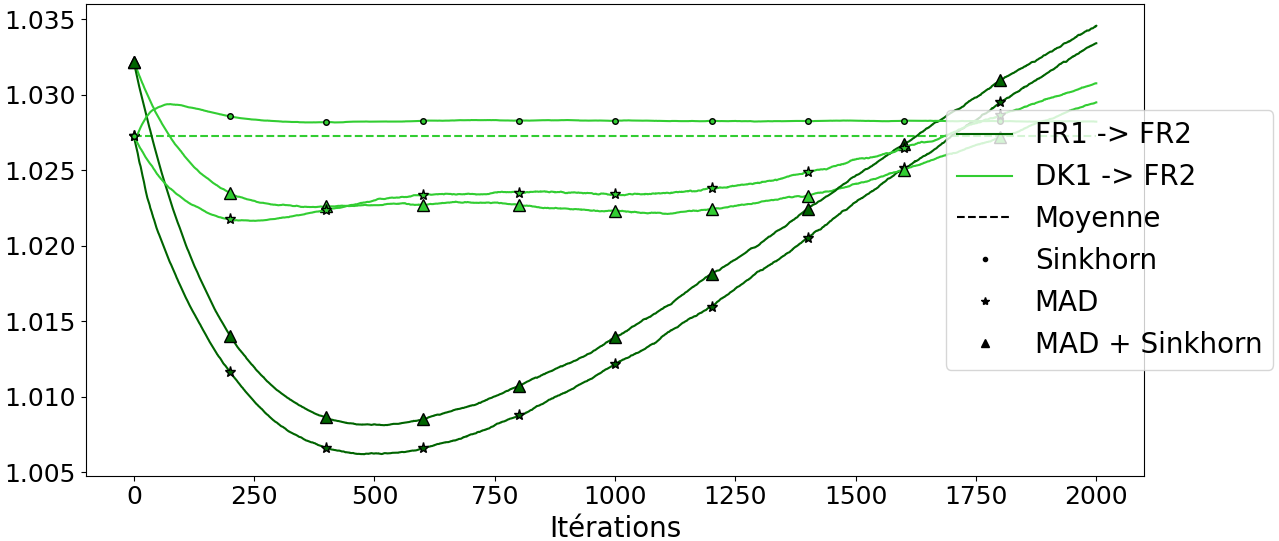
\includegraphics[scale=0.14]{images/80_biais_FR2.png}
		\caption{RMSE en fonction du nombre d'itération avec 80\% de données manquantes}
	\end{minipage}\hfill
    \begin{minipage}[b]{0.4\linewidth}
		\centering 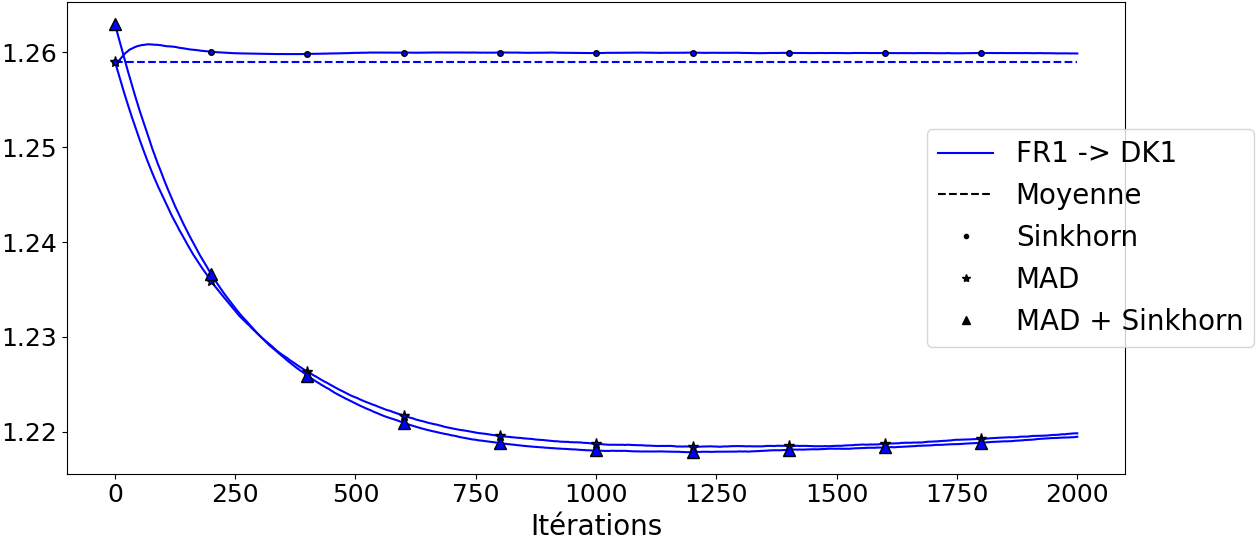
\includegraphics[scale=0.14]{images/80_biais_DK1.png}
		\caption{RMSE en fonction du nombre d'itération avec 80\% de données manquantes}
	\end{minipage}\hfill
    \begin{minipage}[b]{0.4\linewidth}
		\centering 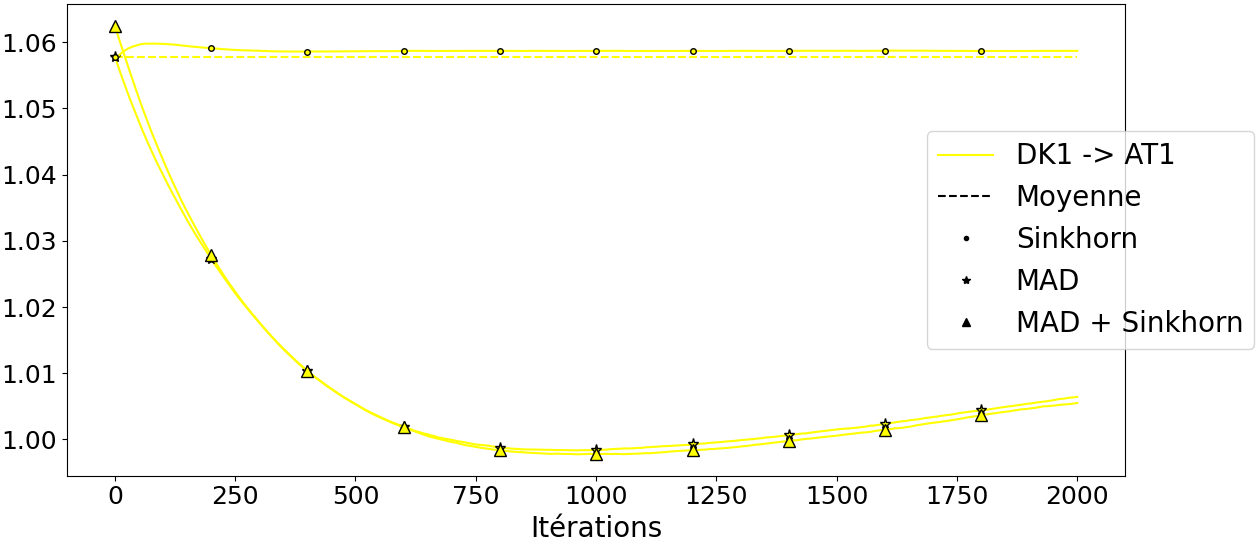
\includegraphics[scale=0.14]{images/80_biais_AT1.png}
		\caption{RMSE en fonction du nombre d'itération avec 80\% de données manquantes}
	\end{minipage}\hfill
    \begin{minipage}[b]{0.4\linewidth}
		\centering 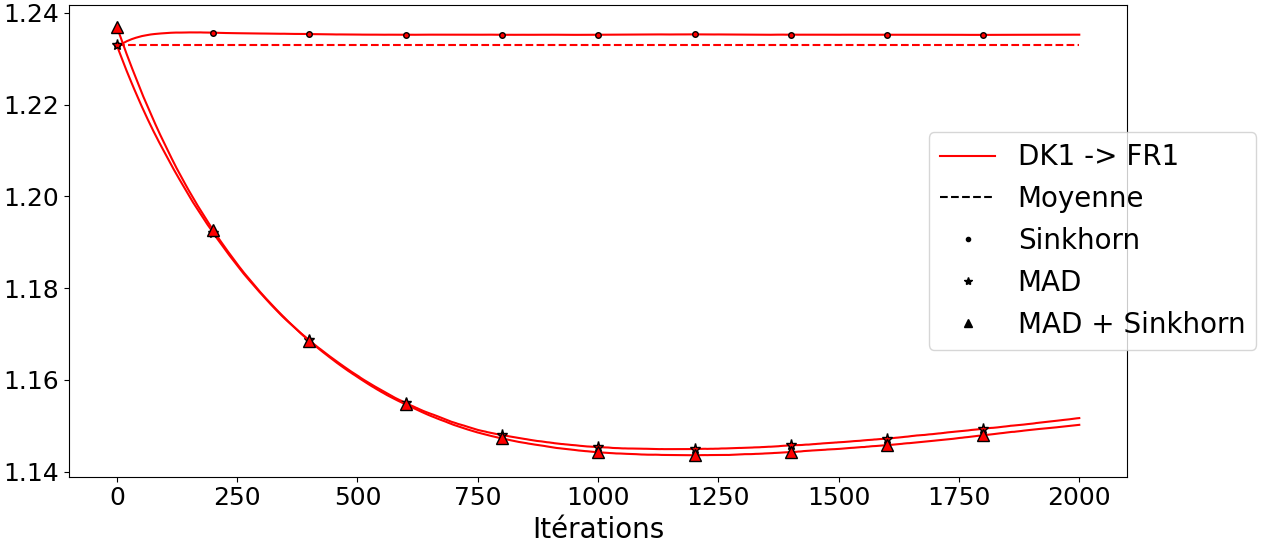
\includegraphics[scale=0.14]{images/90_biais_FR1.png}
		\caption{RMSE en fonction du nombre d'itération avec 90\% de données manquantes}
	\end{minipage}\hfill
    \begin{minipage}[b]{0.4\linewidth}
		\centering 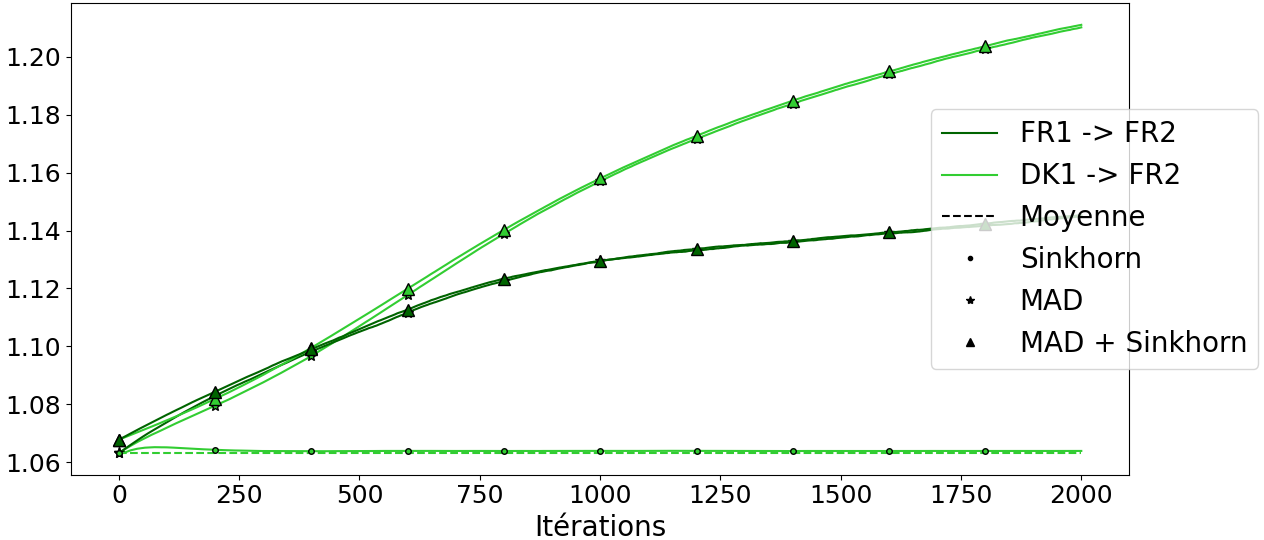
\includegraphics[scale=0.14]{images/90_biais_FR2.png}
		\caption{RMSE en fonction du nombre d'itération avec 90\% de données manquantes}
	\end{minipage}
\end{figure}
\begin{figure}[H]
    \begin{minipage}[b]{0.4\linewidth}
		\centering 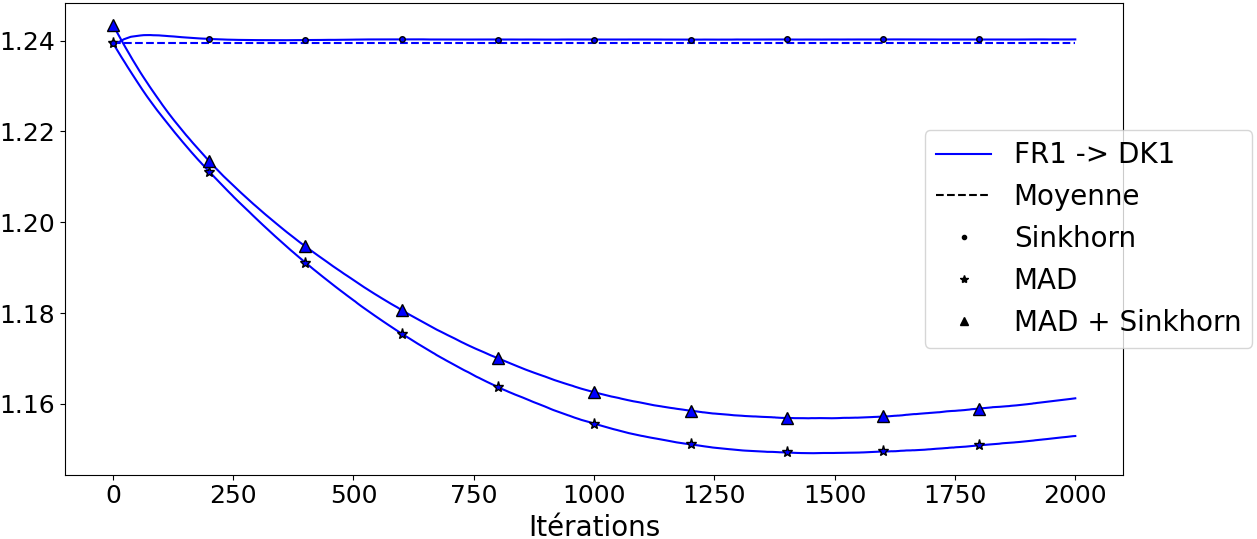
\includegraphics[scale=0.14]{images/90_biais_DK1.png}
		\caption{RMSE en fonction du nombre d'itération avec 90\% de données manquantes}
	\end{minipage}\hfill
	\begin{minipage}[b]{0.4\linewidth}	
		\centering 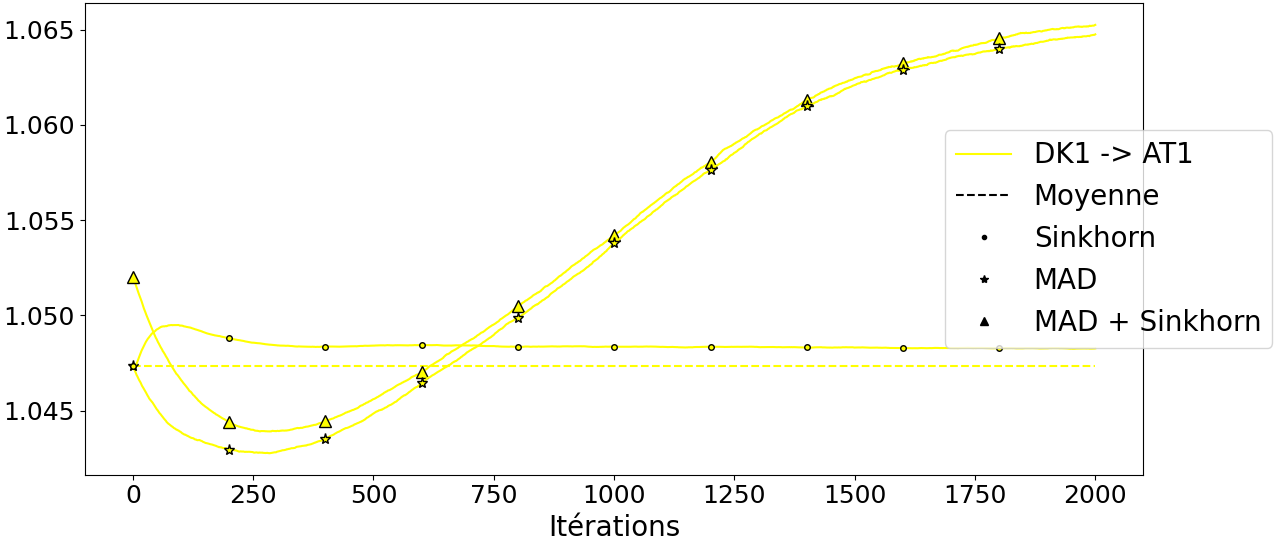
\includegraphics[scale=0.14]{images/90_biais_AT1.png}
		\caption{RMSE en fonction du nombre d'itération avec 90\% de données manquantes}
	\end{minipage}
\end{figure}

\end{document}

